%%%%%%%%%%%%%%%%%%%%%%

\chapter{Person Following}
\label{chapter:person_following}

In this chapter, we focus on one aspect of human-robot interaction, namely person following in an indoor environment. There are many scenarios in which a person following robot can be useful. For example, a robot can carry luggage of travelers in airports, or groceries in a supermarket. Person following is also the enabling capability for interactive acquisition of the \textit{Tour} scenario discussed in Section \ref{sec:tour_scenario}. The robot needs to know how to follow a person before building an environment representation and providing services to the user.  There are two properties a person following behavior should achieve: robust following and social awareness. 

Typically, a service robot operates in a dynamic and populated environment, therefore the robot must be able to keep track of a single person even when they are temporarily occluded. Multimodal person tracking that is presented helps the robot to have better estimates of a user's position. As discussed in Chapter \ref{chapter:multimodal_person_detection_and_tracking}, for the person following task, the robot has to track a designated user, and the detection thresholds of detectors are relaxed for robust tracking at the expense of more false positive detections. 

The robot not only has to keep appropriate distance to the user, but it also has to recognize $what$ the user is trying to accomplish and move accordingly. For example, during the home tour scenario, when the user stops, the robot should predict that the user is going to annotate a landmark, and it should come beside the user instead of standing behind. Moreover, the robot should be smarter when passing doors or following a person who is cutting a corner. In order to be able to handle these scenarios, the robot should act beyond purely reactive following behavior. It is desirable for the robot to anticipate what action the user is likely going to take and act accordingly.

In this chapter, after referring to previous studies on person following robots in Section \ref{sec:following_related_work}, we present the elementary person following method in \ref{sec:following_basic_person_following}. After that, in Section \ref{sec:following_situation_aware} we demonstrate situation awareness of a person following robot in three commonly encountered scenarios: door passing, user activity awareness and handling corners. In Section \ref{sec:following_application_to_telepresence}, we present an application of person following to telepresence robots.

\section{Related Work}
\label{sec:following_related_work}

A robot that follows a person is a widely studied scenario in robotics. A relevant body of work is pursuit evasion \cite{chung2011search}, however the target is trying to evade the follower. In person following robots, we assume that the target is cooperating with the follower.

In one of the earliest works in this area by Sidenbladh \cite{sidenbladh1999person}, robot keeps the person centered in the camera image using a P controller. Prassler \cite{prassler2001motion} also offers a fully reactive approach using the \textit{Velocity Obstacles} concept, which uses the velocity of the target to find allowable velocities of the robot that guarantees avoiding collision if both the target and the robot move with constant speed. The approach is applied on a wheelchair, even though social constraints were not considered. 
The robot does not necessarily follow a person directly from behind. Gockley \cite{gockley2007developing} observed how people walk together. It is reported that partners who were conversing tend to look forward with occasional glances to each other. Ohya \cite{ohya2002intelligent} presents a following method to escort a target on the side while avoiding obstacles. It was assumed that the target would move with the same acceleration and velocity. Murakami \cite{murakami2014destination} presents a method to first estimate the sub-goal of the leading person and then following as if the robot knows the goal. 

Park \cite{park2013autonomous} models the problem as a control problem and offers an algorithm based on Model Predictive Control.
\cite{miura2010development} employs randomized tree expansion and biases the calculated paths towards a sub-goal, which is the current position of the person. Hoeller \cite{hoeller2007accompanying} adopts the virtual targets idea and selects a goal position in a circular region around the person. Stein \cite{stein2013navigating} proposes choosing and following a leader to handle navigation in crowds.

Some of the relevant works considered the social side of the interaction. Gockley compared two elementary following methods: direction following, where the robot always attempts to drive towards the tracked person, and path following, where the robot follows the path the person took. It was shown that direction following behavior was perceived as more human-like and natural than path following. Yuan's \cite{yuan2008spatial} system switches following behavior between parallel following, direction and path following depending on the layout of the obstacles. Zender \cite{zender2007human} emphasizes on situation awareness for following and studies cases of handling doors and corridors. To handle the doors, the robot increases its following distance and that leads the robot to wait for a while. Following in a corridor is handled with an approach similar to Pacchierotti \cite{pacchierotti2005human}, and the robot's speed is increased. \cite{loper2009mobile} presents a system that is capable of responding to verbal and non-verbal gestures and follow a person. When following a group of people, a common method is to choose and follow a leader. Granata \cite{granata2012framework} presents behaviors such as going towards, following and searching a user. Ota \cite{ota2013recovery} touches upon the recovery functions whenever the robot loses tracks of the leading person.

\section{Basic Person Following}
\label{sec:following_basic_person_following}

In this section, we describe our basic person following method. To keep track of the person

When the following behavior is initiated from a higher level process, first the person to be followed must be tracked. The robot looks for the closest person in the vicinity of the robot (within $2m$). If no person is detected for some time, then the command is invalidated. We use the person detection and tracking system described in Section \ref{chapter:multimodal_person_detection_and_tracking}.

\begin{figure}[ht!]
\hspace*{4cm} 
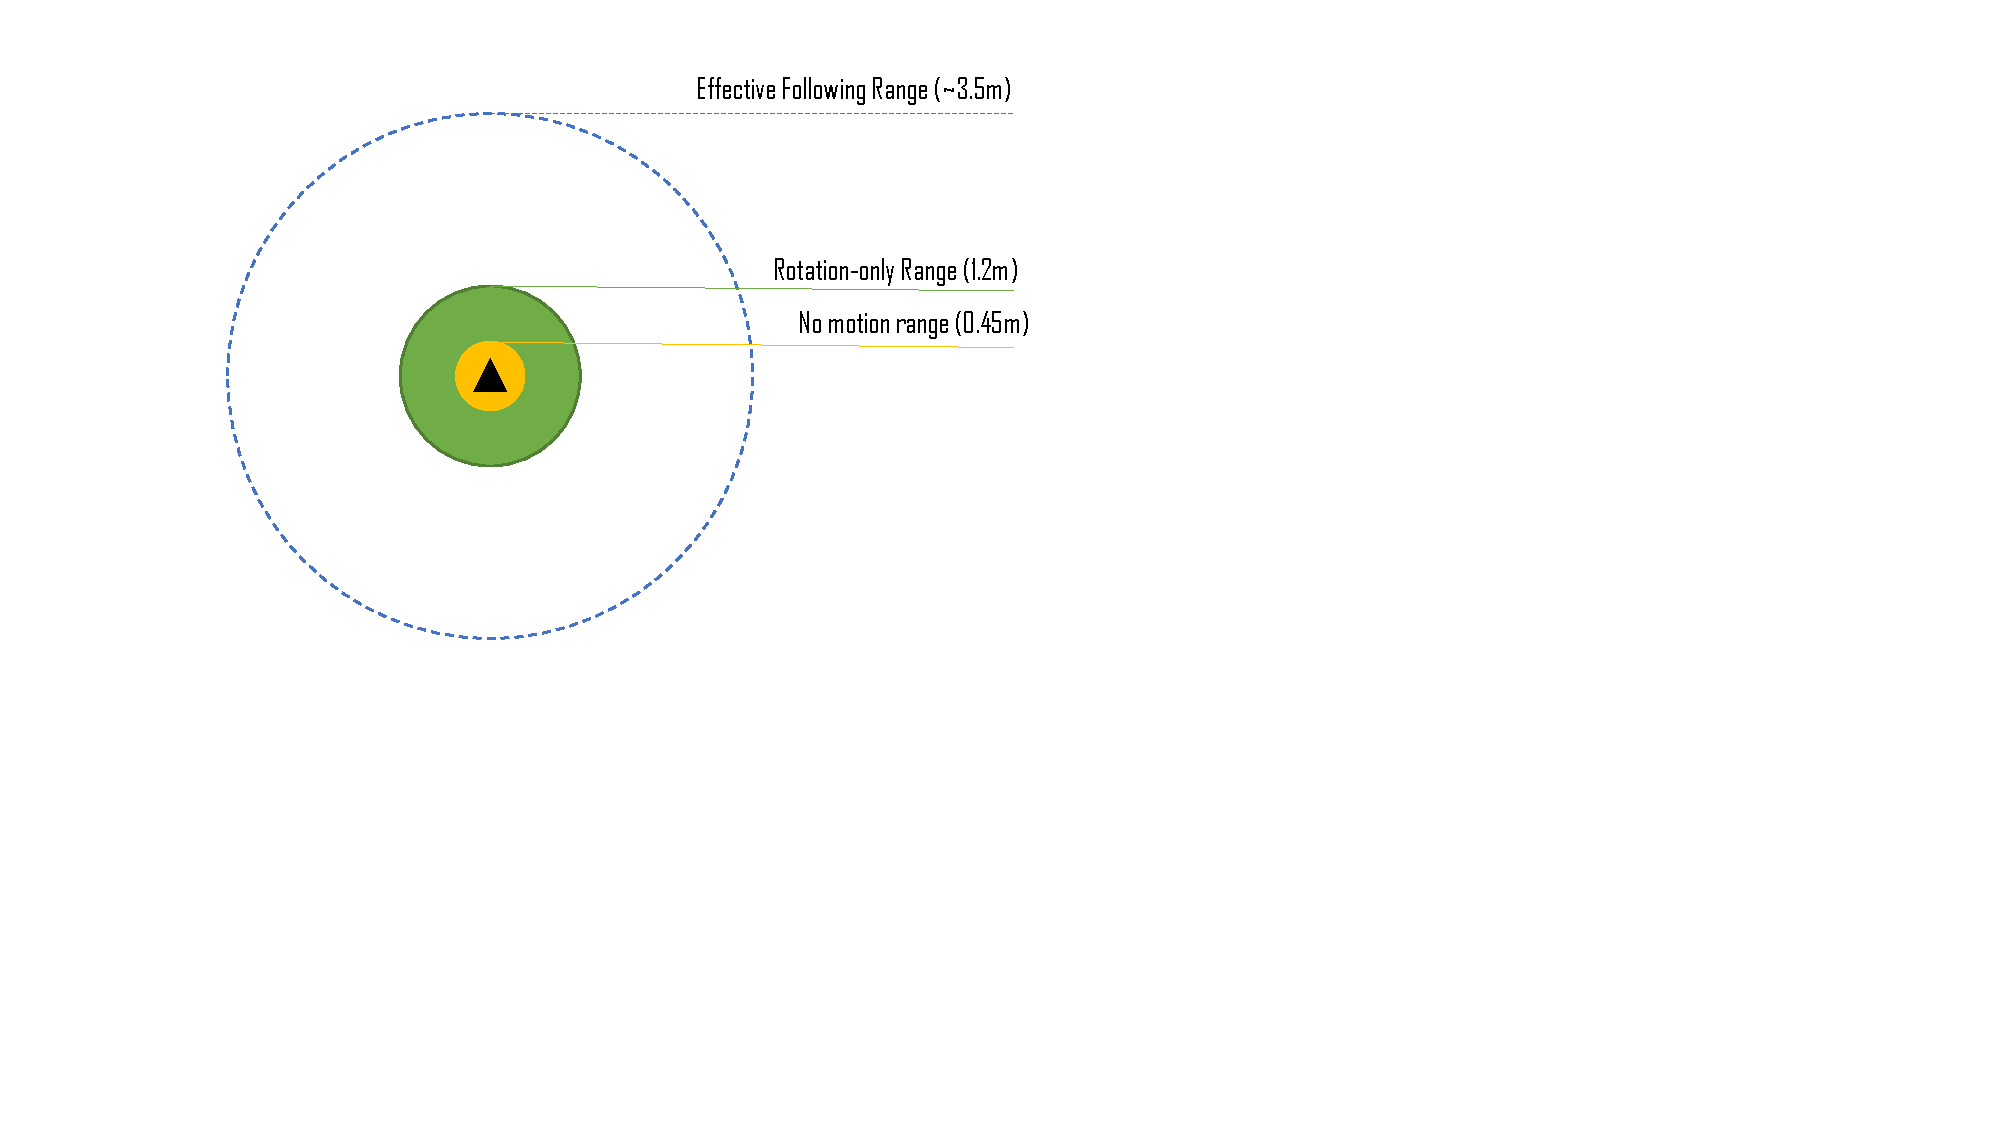
\includegraphics[width=0.7\textwidth]{pics/following_ranges_cropped}
\caption{Overhead view of relevant ranges for person following. Robot is represented as the triangle in the middle.}
\label{fig:following_ranges}
\end{figure}

In the basic person following mode, the robot has three different strategies depending on the distance towards the followed person. The distance to the user is calculated as the distance from the center of the robot base to the person's current location estimation. We used Hall's characterization of personal spaces in order to determine the distance limits. See Section \ref{sec:personal_spaces} for a review of Hall's work. The three distinct zones and corresponding robot behavior are given as follows:

\textbf{Intimate Zone $[0-0.45m]$:} In this short interval, the person is very close to the robot, therefore any motion of the robot may be potentially unsafe. Therefore the robot comes to a complete halt in this zone ($v=0,w=0$). This behavior also allows the user to safely interact with the on-board User Interface.

\textbf{Personal Zone $[0.45-1.2m]$:} When the robot is in the personal zone of the user, the robot stops and only rotates towards the followed person ($v=0,w=w_{rotation}$). The rotational velocity is determined with a P controller, with the error term defined as the difference between the current orientation and the tracked person's orientation. The rotational velocity is capped at a fixed value, so that the person feels comfortable with the rotation of the robot.

\begin{figure}[h!]
\centering
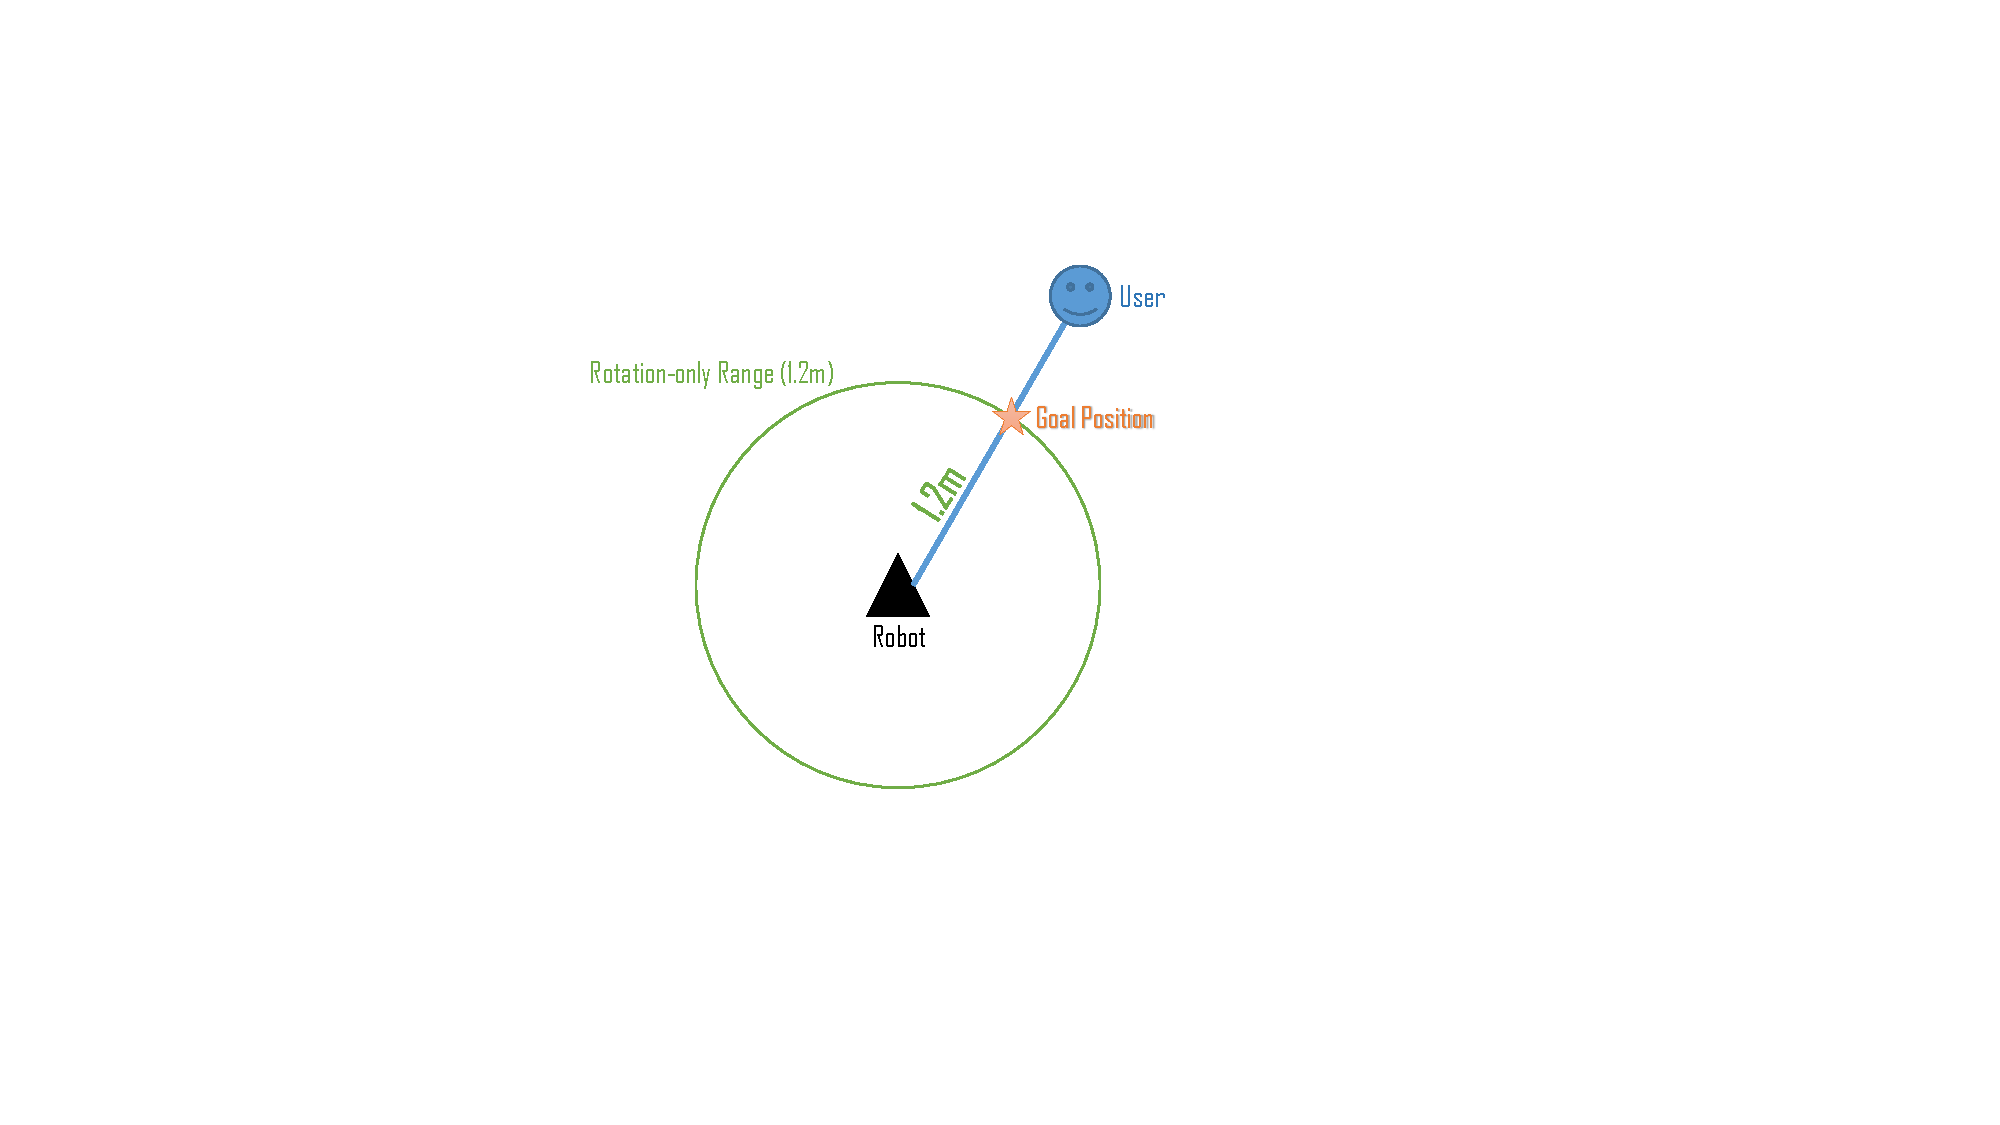
\includegraphics[width=0.55\textwidth]{pics/following_1m_cropped}
\caption{An illustration of how the goal position is calculated when the user is in the social space $[1.2m-3.5m]$.}
\label{fig:following_1m}
\end{figure}

\textbf{Social Zone $[1.2m-3.5m]$: } In this range interval, the robot executes the main following behavior. At every time step, a goal pose that is $1.2m$ away from the and headed towards the user is calculated, see Figure \ref{fig:following_1m} for an illustration. A collision-free path is found and the robot executes this path until a new measurement from the tracked person is received. The path is found using Dynamic Window Approach (DWA) local planing method. We use the ROS implementation of DWA for the basic following behavior.

Sometimes it is inevitable that the person tracking system loses the target, particularly when the person is consistently faster than the robot or the person goes outside the range of the sensors (further than $\sim3.5m$ in our case). When this happens, the robot will attempt to go to its last calculated goal position and look for the person. By this means, the robot attempts to keep up with the lost person as far as possible with the hope that the person will re-appear in the vicinity of the last seen position. After the robot reaches this goal, it stops and waits for an amount of time. If the user is saved to the database, or the robot already knows that he/she is in the database, then the face recognition system described in Section \ref{sec:multimodal_face_recognition} is activated. Otherwise, the robot continues following the closest person that appears in this position. If no person is detected within a fixed amount of time, $5$ seconds in our implementation, then the robot declares that the person is lost.


\section{Situation Awareness For Person Following}
\label{sec:following_situation_aware}

Most simply put, \textit{Situation Awareness (SA)} is knowing what is going on around you. Endsley \cite{endsley2000situation} defines three steps for SA: Perception is detecting the situation by perceiving cues, comprehension is combining and interpreting information and projection is forecasting future events.

In this section, we discuss SA for person following behavior for mobile robots. In the previous section, we presented the basic following behavior, where the robot follows the person from behind, while maintaining a fixed distance. The related works on person following discussed in Section \ref{sec:following_related_work} uses the same principle: the robot uses the person to calculate the target position and blindly follows the human irrespective of the situation. Although this method is sufficient for some scenarios, it can easily lead to socially awkward situations. For example, consider for a person following robot that its users stops just outside a door. In this case, the robot would occupy the doorway, blocking other people's passage, however thinks it is doing its task well because it maintains its distance to the user. If the robot knows what the person intends to do, it can anticipate those actions and suitably adjust its behavior.

Person following can be used in different contexts, such as for carrying luggage in airports or groceries in a supermarket. We showed in Chapter \ref{chapter:map_annotation} that semantic maps that include landmarks and waypoints could be to communicate goals between the robot and the user.  The stored semantic information can also be used to facilitate robot navigation. We focus on demonstration of SA for the Tour Scenario and specifically for the person following behavior.

Our method for utilizing SA for person following is via triggered events. Handling of an event during following is implemented as a sequence of four phases:

\begin{enumerate}
\item Signal: Robot detects an event using perceptual cues
\item Approach: Robot moves to a position better suited to the task
\item Execution: Robot and Human interacts for the task
\item Release: Robot detects the end of event
\end{enumerate}

When the event ends, robot continues with Basic Following behavior described in Section \ref{sec:following_basic_person_following}. With this methodology, robot uses the three steps of SA: Perception for detecting the start and ending of an event, Comprehension for interpreting where it should move to and what the task is, and Projection to estimate the future goals of the person. We will study the following events: how should the robot move when the user is showing landmarks in Section \ref{sec:following_landmark_labeling} and how it should handle passage of doors in Section \ref{sec:following_door_passing}.

%As another example, if the guiding person stops and chats with another person, it may be an awkward situation for the robot to wait while facing the back of its user. It may be socially more appropriate for the robot to join the group.


\subsection{Landmark Labeling}
\label{sec:following_landmark_labeling}

One of the problems during the Tour Scenario is that as the robot is following the user, it does not have any information about the task. This leads to awkward situations when the user wants to label a landmark or object, because the robot can not perceive the pointing gesture or the object/landmark of interest when it is following from behind all the time. The robot behavior can be more intelligent in those cases if the robot can predict ahead of time when the user is going to annotate map features. That way, the robot can demonstrate SA.

\begin{table}[ht!]
	\centering
  \begin{tabular}{l |  m{10cm}}    
    \toprule    
    Signal & {$dist(user, convex hull(landmark))<threshold$}\\       
	                           & {$speed(user)\sim 0$} \\
	                           & {person roughly facing landmark}\\ \midrule		                           		                                
    Approach & {Optimal Goal: Close to both the landmark and person, facing in between}\\       \midrule
    Execution & {User points and labels landmark}\\  \midrule
    Release & {$dist(user, convex hull(landmark))>threshold$}\\ 
    \bottomrule
  \end{tabular}
      \caption{Conditions to trigger phases when the user is involved with the Landmark Labeling Event during following.}
    \label{table:situation_aware_list_landmark}
\end{table}


\begin{figure}[ht!]
\centering
%
        \subfigure[]{%           
           \label{fig:situtation_aware_landmark_labeling0}
           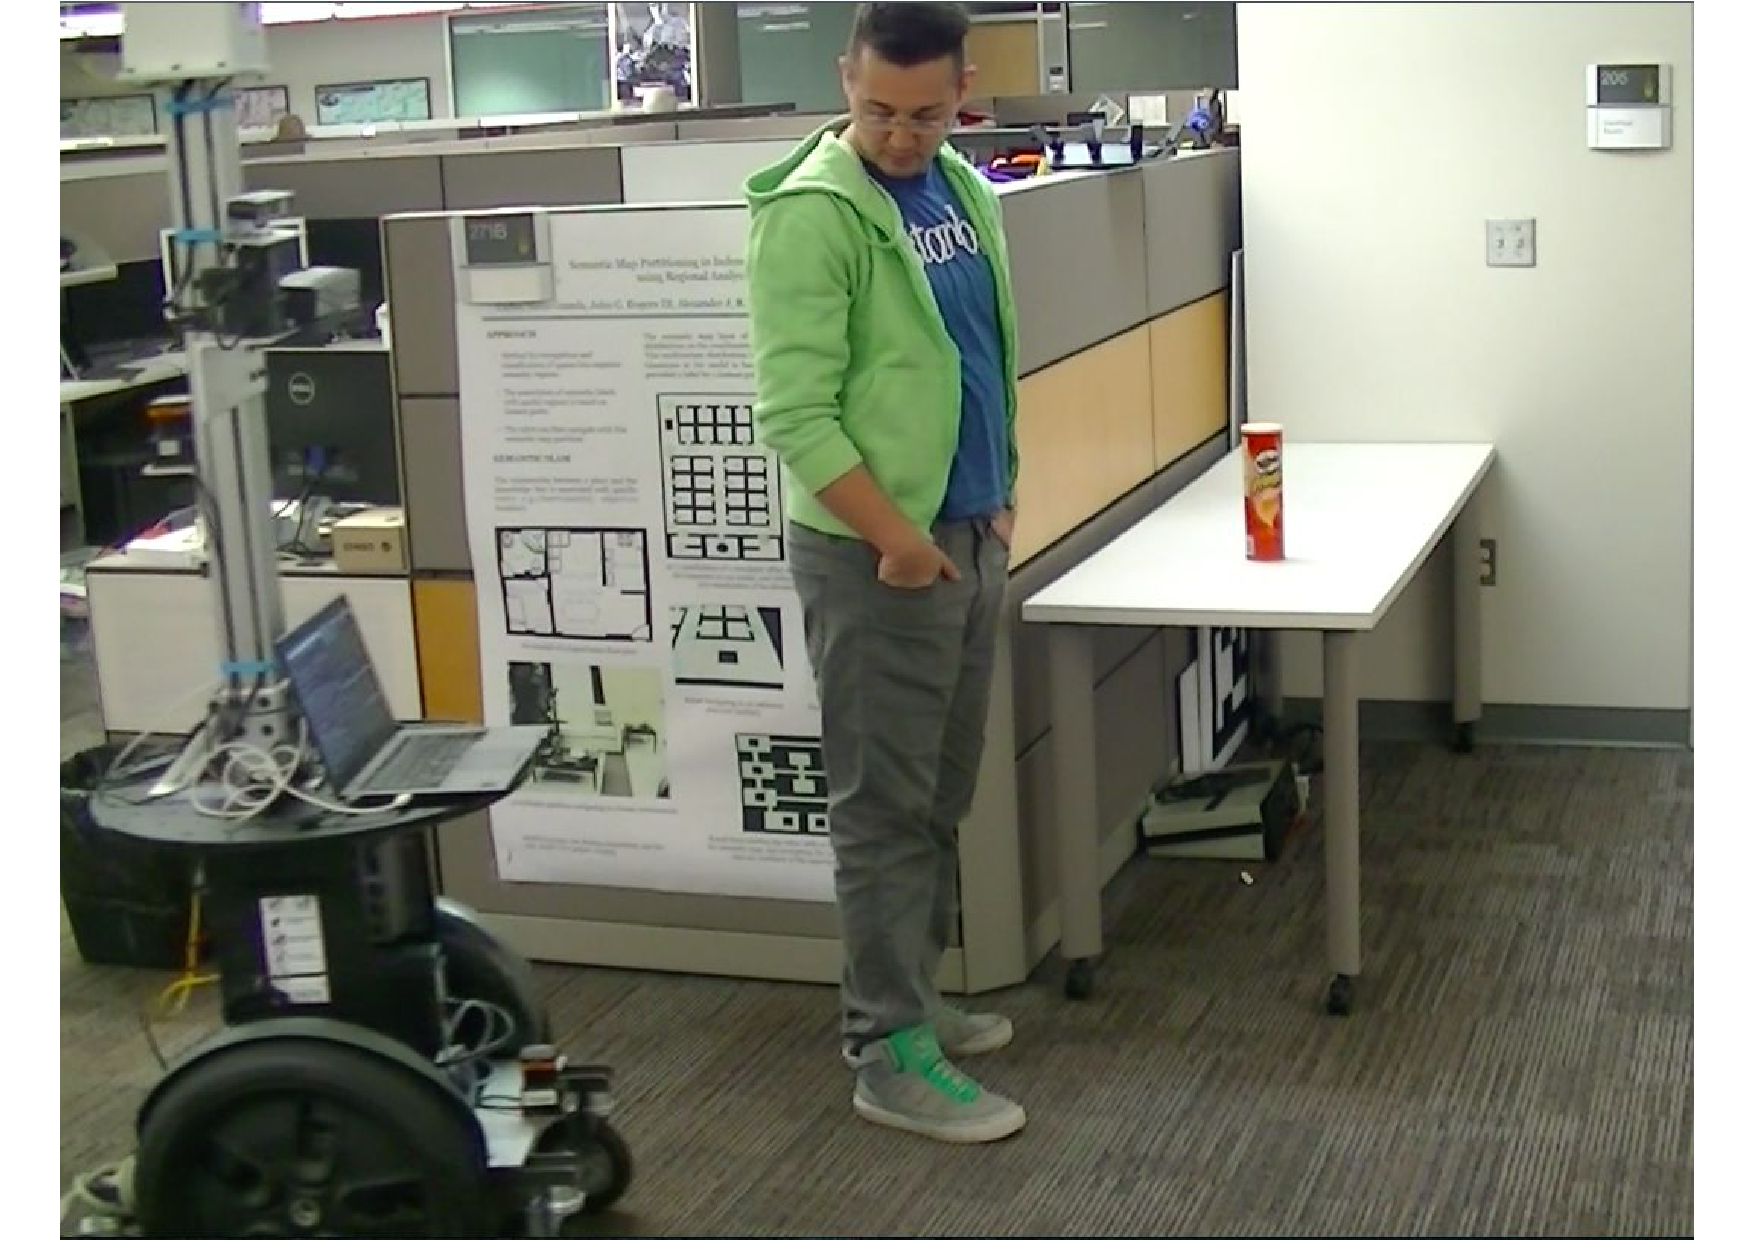
\includegraphics[width=0.475\textwidth]{pics/sit_table_00}
        } 
         \subfigure[]{%           
           \label{fig:situtation_aware_landmark_labeling2}
           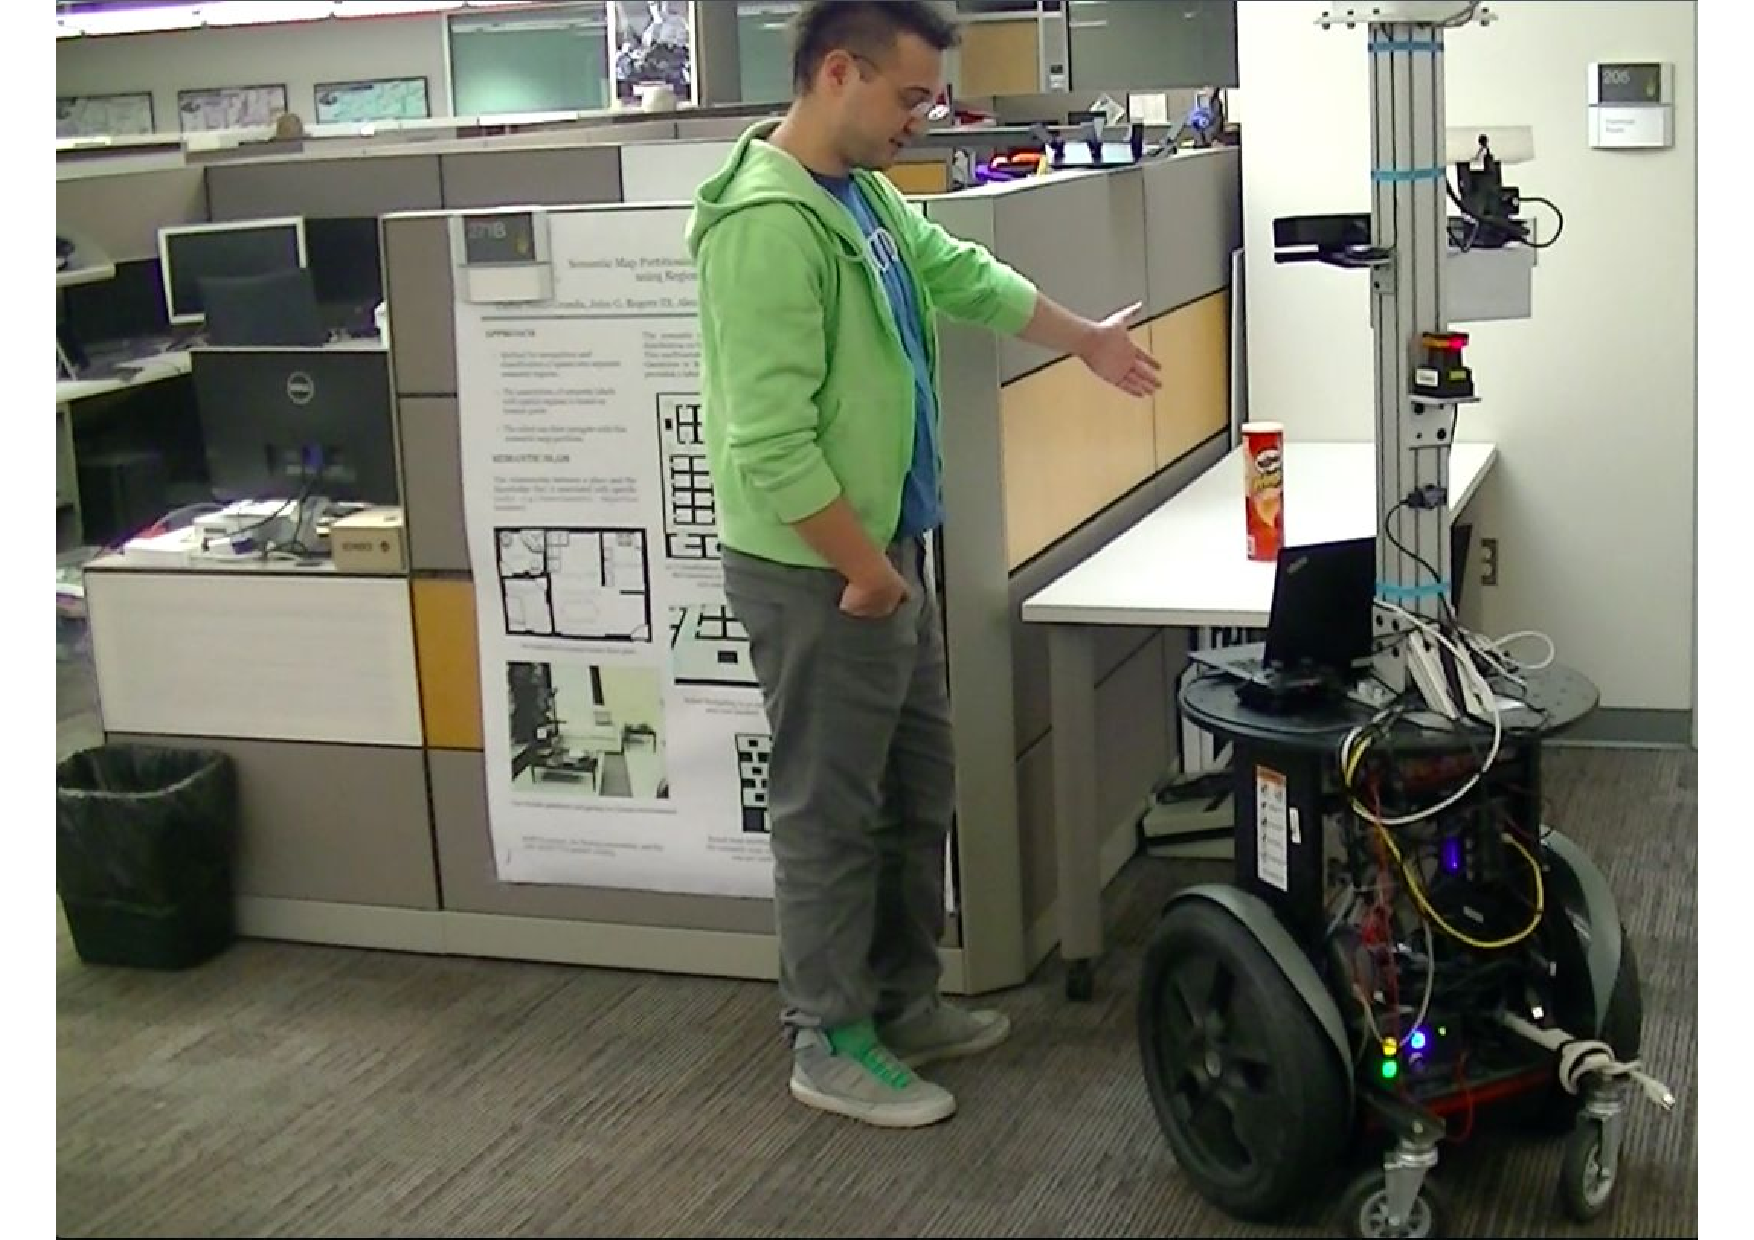
\includegraphics[width=0.48\textwidth]{pics/sit_table_02}
        } \\
        \subfigure[]{%
        	\label{fig:situtation_aware_landmark_labeling3}
            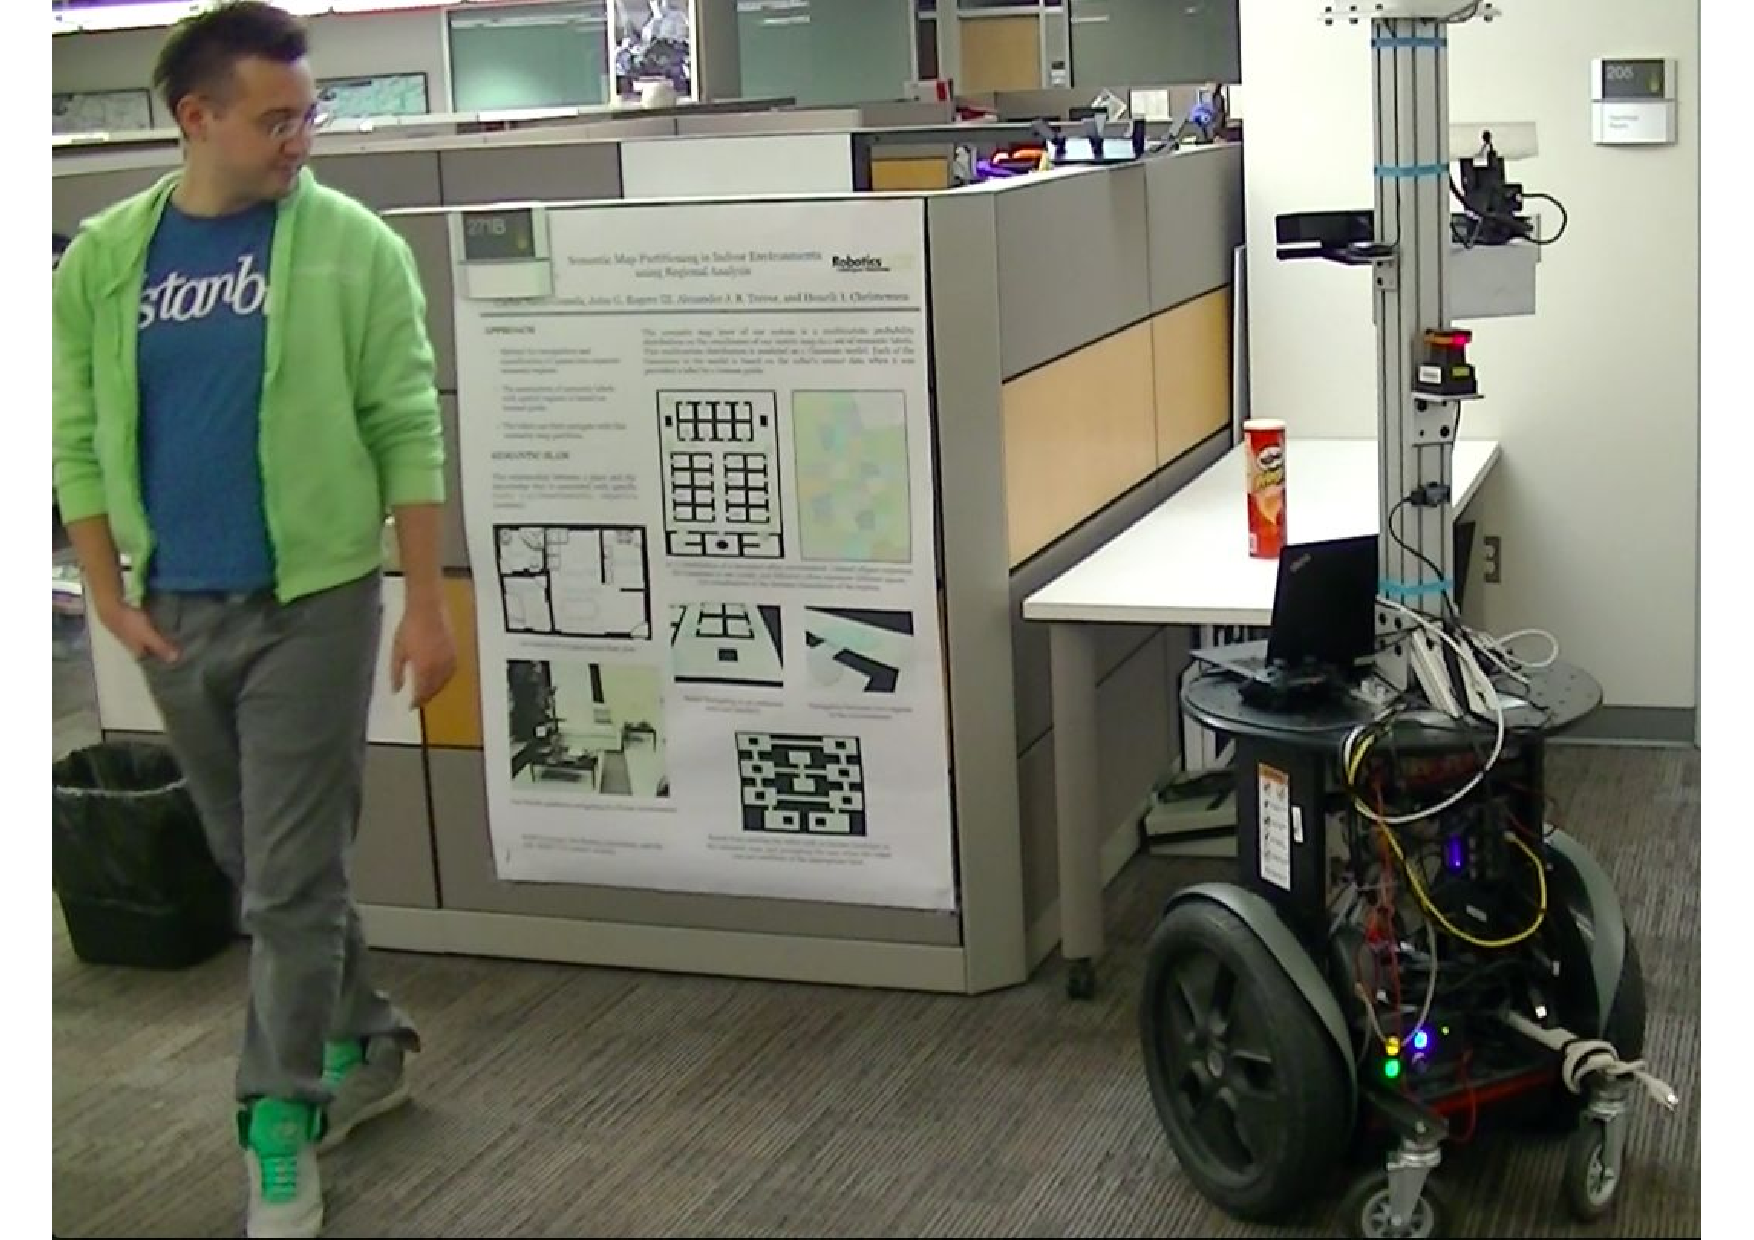
\includegraphics[width=0.48\textwidth]{pics/sit_table_03}
        }%\\        
        \subfigure[]{%           
           \label{fig:situtation_aware_landmark_labeling4}
           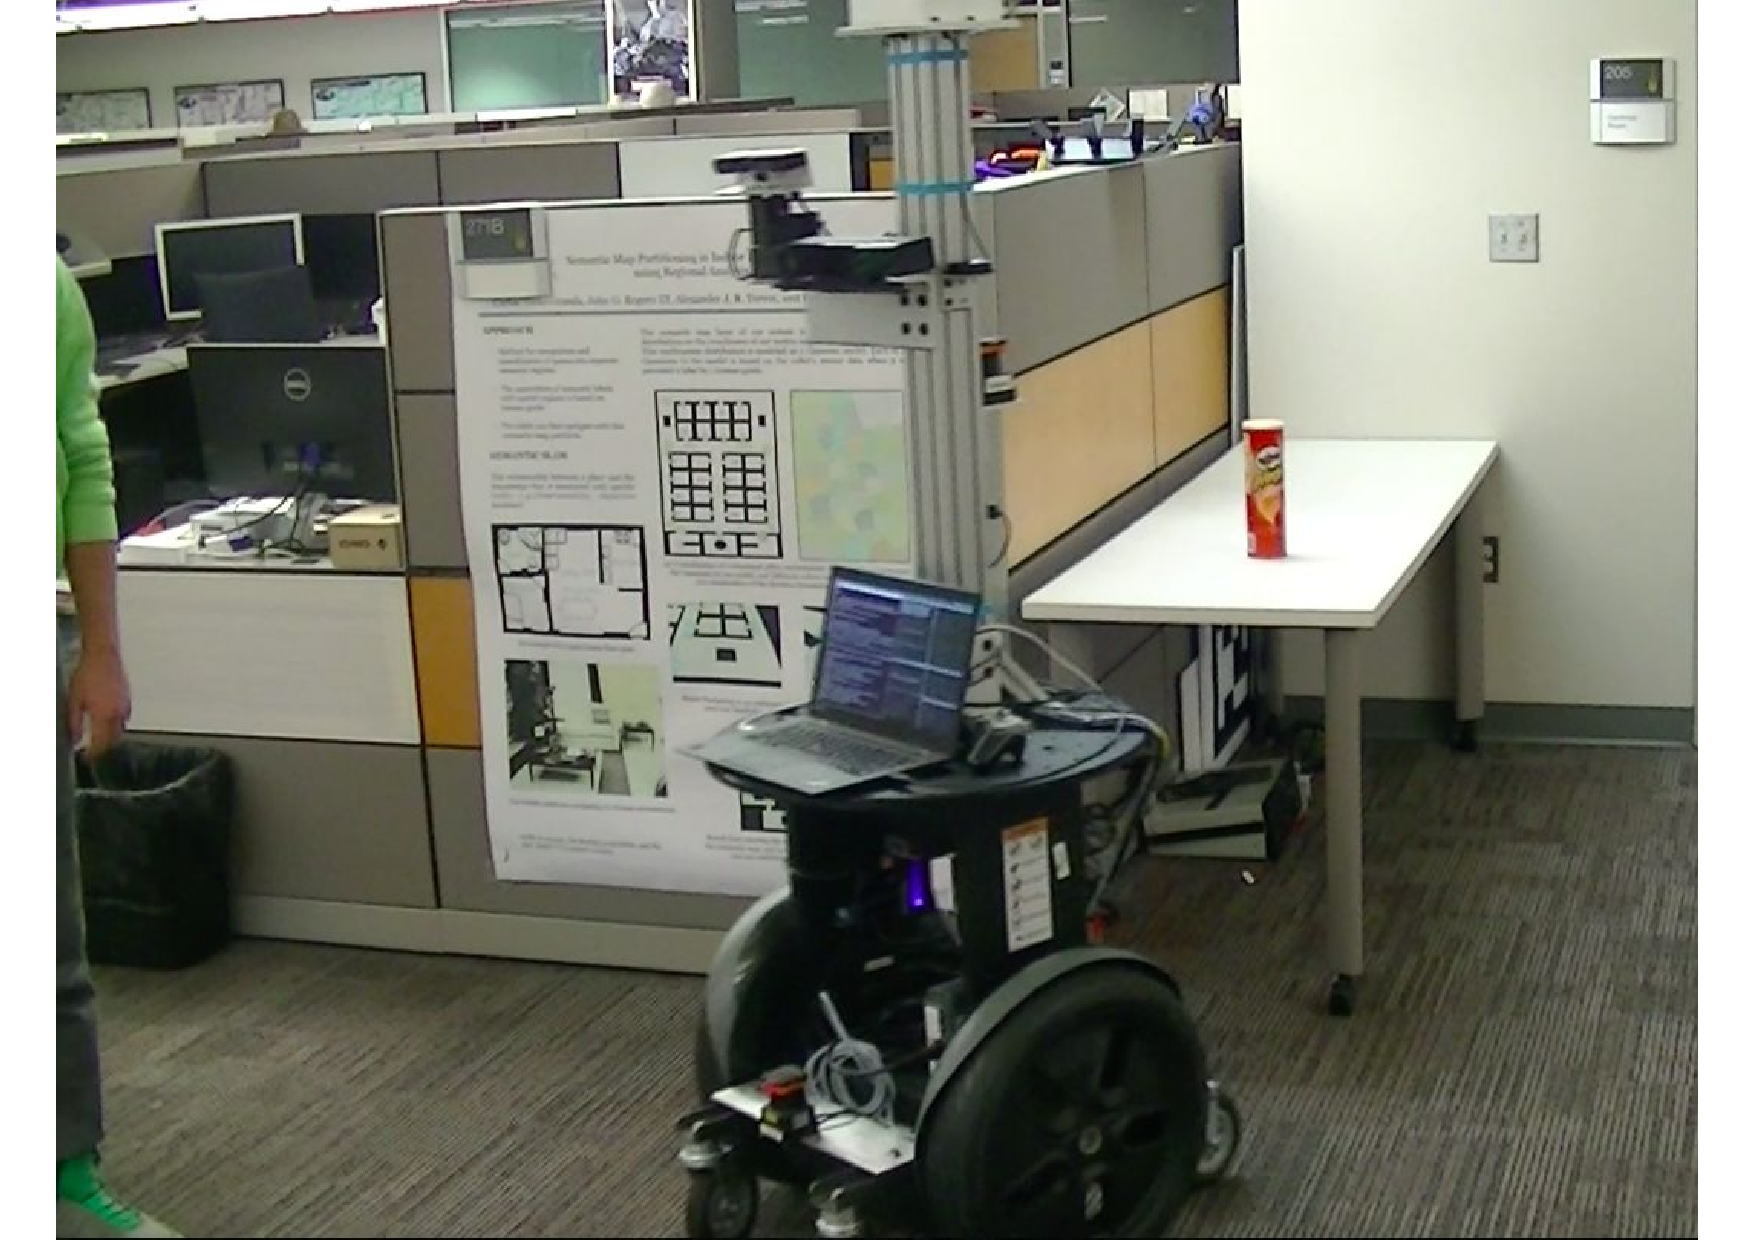
\includegraphics[width=0.49\textwidth]{pics/sit_table_04}
        }
    \caption{Demonstration of situation awareness for the Tour scenario. The robot is following the user throughout the environment and keeping a fixed distance of 1m to the user. a) Signal phase: The user has stopped and is in the cloxe proximity to the convex hull of the table. b) Approach phase: The robot calculates and navigates to a goal position, so it can perceive the pointing gesture and target. Execution phase: The user points out to the object on the table. c) Release phase: user moves away from the table d) Basic following behavior continues.}
   \label{fig:situtation_aware_landmark_labeling}
\end{figure}

Our approach relies on detecting whenever labeling is going to happen, and position the robot base so it has a better chance to perceive both the pointing gesture and the object/landmark of interest. We follow the Signal/Approach/Task/Release procedure for the design of this behavior. The Signaling phase is triggered whenever the user is nearby a detected landmark or object and facing it. The user must be at full stop to enable signaling for this behavior, because the user may also walk past the landmark. After the robot detects the signal, we sample positions around the human to locate a ``suitable" goal pose. We use a utility function that scores candidate goal points. Intuitively, a pose that is close both to the landmark and person and could see both entities is considered a suitable goal pose. We sample points $360^{\circ}$ around the position of the user, for a fixed sampling resolution. Every sampled position $p$ has a score of:
\[
Score(p) = 1.0 - Cost_{visibility}(p) - Cost_{obstacle}(p)
\]
Where we define the costs as:
\begin{align} 
\begin{split} 
Cost_{visibility}(p)&=dist(user,landmark)/(dist(p,landmark)-dist(p,user)) \\
Cost_{obstacle}(p)&=max( local\_cost(p),global\_cost(p))
\end{split} 
\end{align}



The local and global costs are fetched from the ROS costmaps, normalized to [0.0-1.0] interval. The sample with the highest nonnegative score is chosen as the goal position. The orientation of the robot is chosen as looking at the center between the user's position and the landmark's position. After the goal pose is determined, the robot is commanded to navigate there. Then the user can execute the labeling task via pointing gestures. After the task is completed, the robot looks for the user to leave the landmark area. When the robot detects that the user intends to leave by checking the distance to the landmark, it continues the Tour scenario by continuing to follow the user. If, at any time during the phases, the person tracking fails, it informs the user so following can be restarted. The phases and conditions for this behavior are summarized in Table \ref{table:situation_aware_list_landmark}. The situation awareness for labeling landmarks is implemented on the Segway robot for the Tour Scenario. The phases can be seen in Figure \ref{fig:situtation_aware_landmark_labeling}.

%\subsection{Joining the Group}
%\label{sec:following_joining_group}
%
%Join Group
%
%\begin{figure}[ht!]
%\centering
%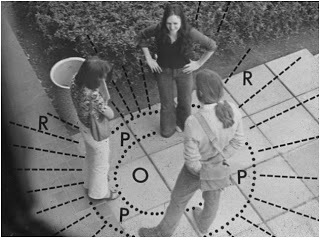
\includegraphics[width=0.5\textwidth]{pics/f_formation}
%\caption{Kendon's F-Formation studies how people arrange themselves within a group}
%\label{fig:f_formation}
%\end{figure}
%
%Phases
%
%\begin{table}[H]
%	\centering
%  \begin{tabular}{l |  m{10cm}}    
%    \toprule    
%    Signal & {$dist(user, otherperson)<threshold$}\\       
%	                           & {$velocity(user)\sim 0$} \\
%	                           & {$velocity(otherperson)\sim 0$} \\ \midrule		                           		                                
%	    Approach & {Optimal Goal: inside $p \textendash space$ of the group, looking to center of the group}\\       \midrule
%    Execution & {Robot communicates with people, receives commands}\\  \midrule
%    Release & {$dist(user,otherperson)>threshold$}\\ 
%    \bottomrule
%  \end{tabular}
%      \caption{Conditions to trigger phases when the guiding user stops and interacts with another person during following.}
%    \label{table:situation_aware_list_group}
%\end{table}
%with a process similar to the one described in Section \ref{sec:following_landmark_labeling}. The candidate points, however 

\subsection{Door Passing}
\label{sec:following_door_passing}

When the user approaches a door during following, the situation can easily become problematic if the robot continues with the basic person following behavior. For example, if the user intends to close an open door or open a closed door, the robot might end up blocking the movement of the door. Moreover, a deadlock situation occurs when the user wants to go through a door with spring-loaded hinges. In that case, the user would need to hold to door to keep it open, and because the distance between the robot and the user is less than the threshold, the robot would stay still and won't pass the door. A robot SA should be aware of this possibility and take appropriate action. 

\begin{table}[H]
	\centering
  \begin{tabular}{l |  m{10cm}}    
    \toprule    
    Signal & {$dist(user, convexhull(door))<threshold$}\\         
    	      & {$speed(user)\sim 0$} \\
	      & {User performs pointing gesture towards the passage}\\ \midrule	                           
    Approach & {Optimal Goal: A position on the other side of the door that doesn't block the doorway}\\       \midrule
    Execution & {User also passes the door}\\  \midrule
    Release & {$dist(user, convexhull(door))>threshold$ }\\ 
    \bottomrule
  \end{tabular}
      \caption{Conditions to trigger phases when the user is passing through a door during following.}
    \label{table:situation_aware_list_group}
\end{table}

\begin{figure}[ht!]
\centering
%
        \subfigure[]{%           
           \label{fig:situtation_aware_door_passing0}
           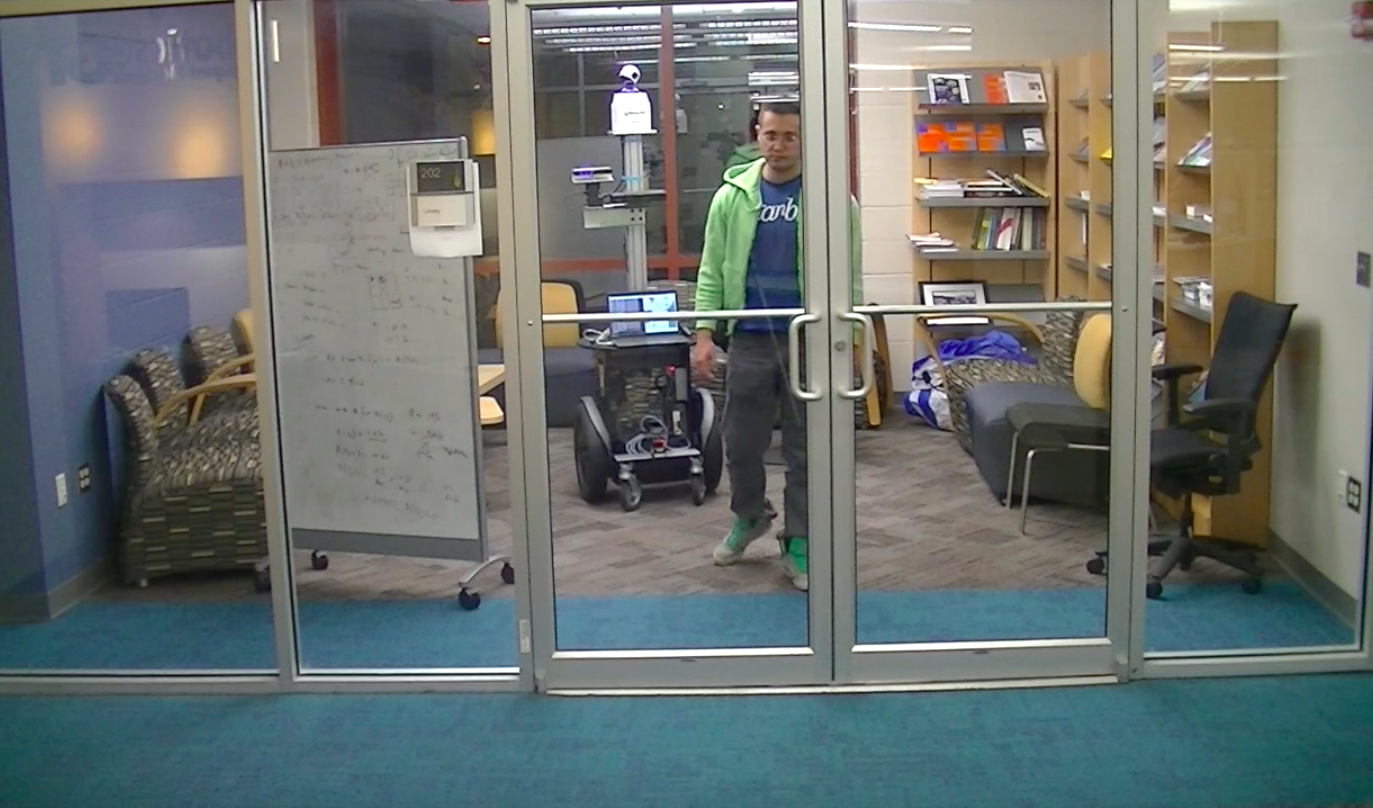
\includegraphics[width=0.475\textwidth]{pics/sit_door_00}
        } 
        \subfigure[]{%           
           \label{fig:situtation_aware_door_passing1}
           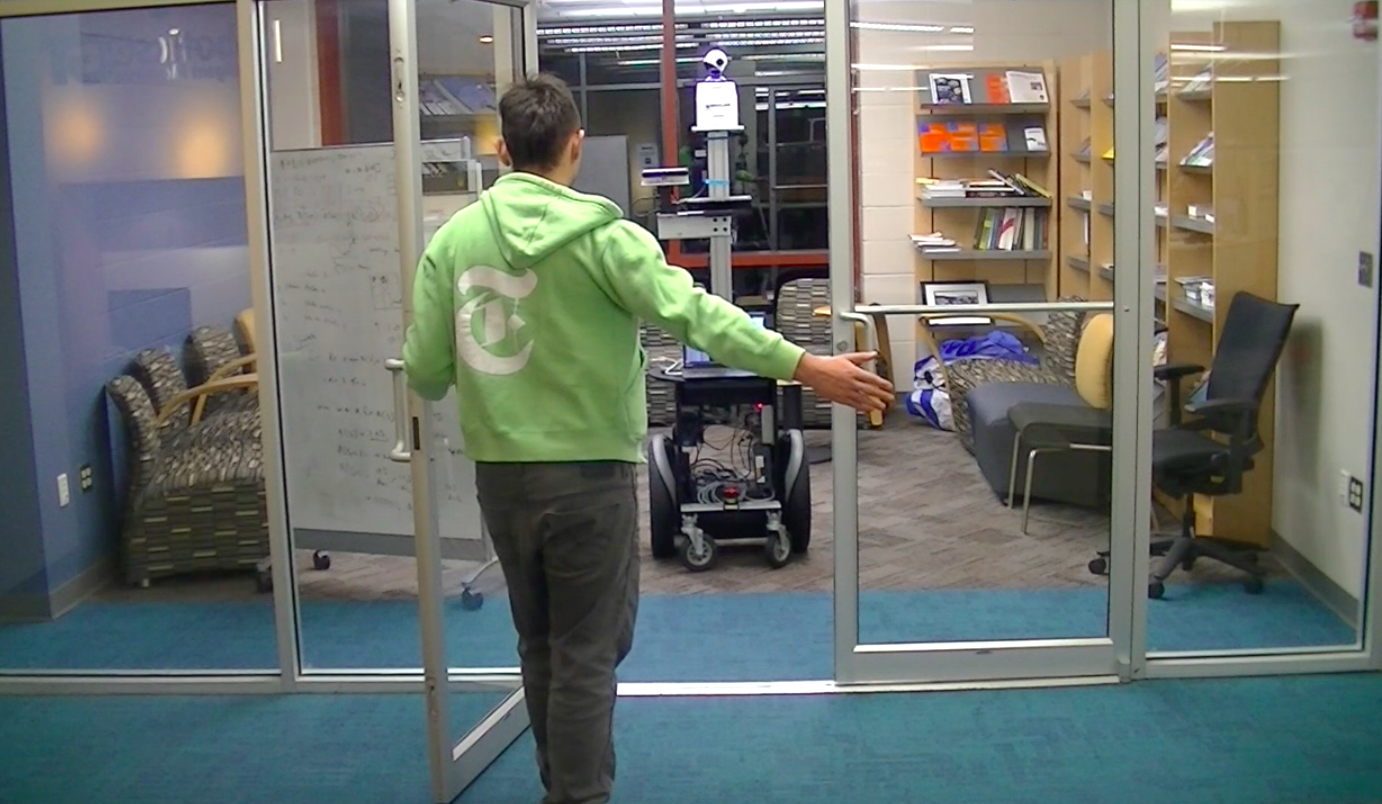
\includegraphics[width=0.48\textwidth]{pics/sit_door_01}
        } \\
        \subfigure[]{%
        	\label{fig:situtation_aware_door_passing2}
            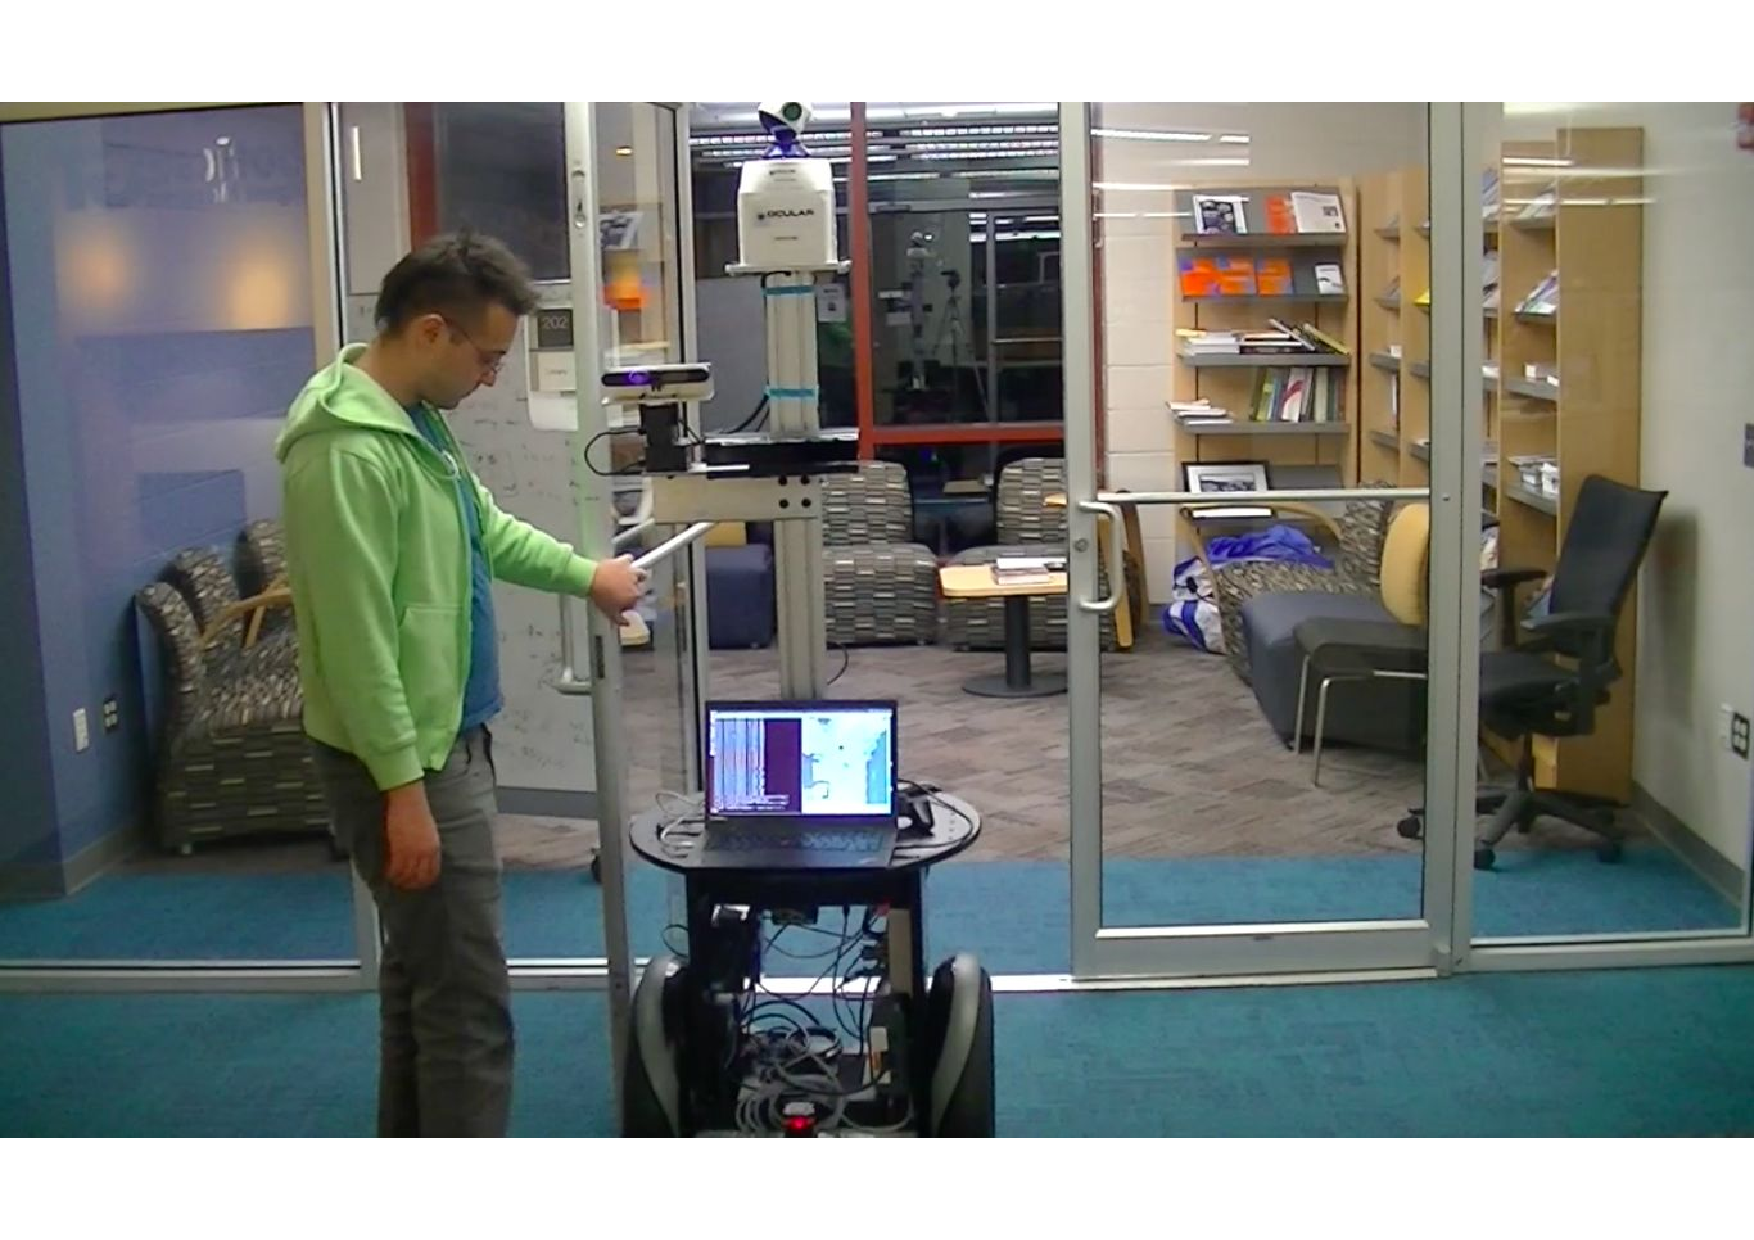
\includegraphics[width=0.48\textwidth]{pics/sit_door_03}
        }%\\        
        \subfigure[]{%           
           \label{fig:situtation_aware_door_passing3}
           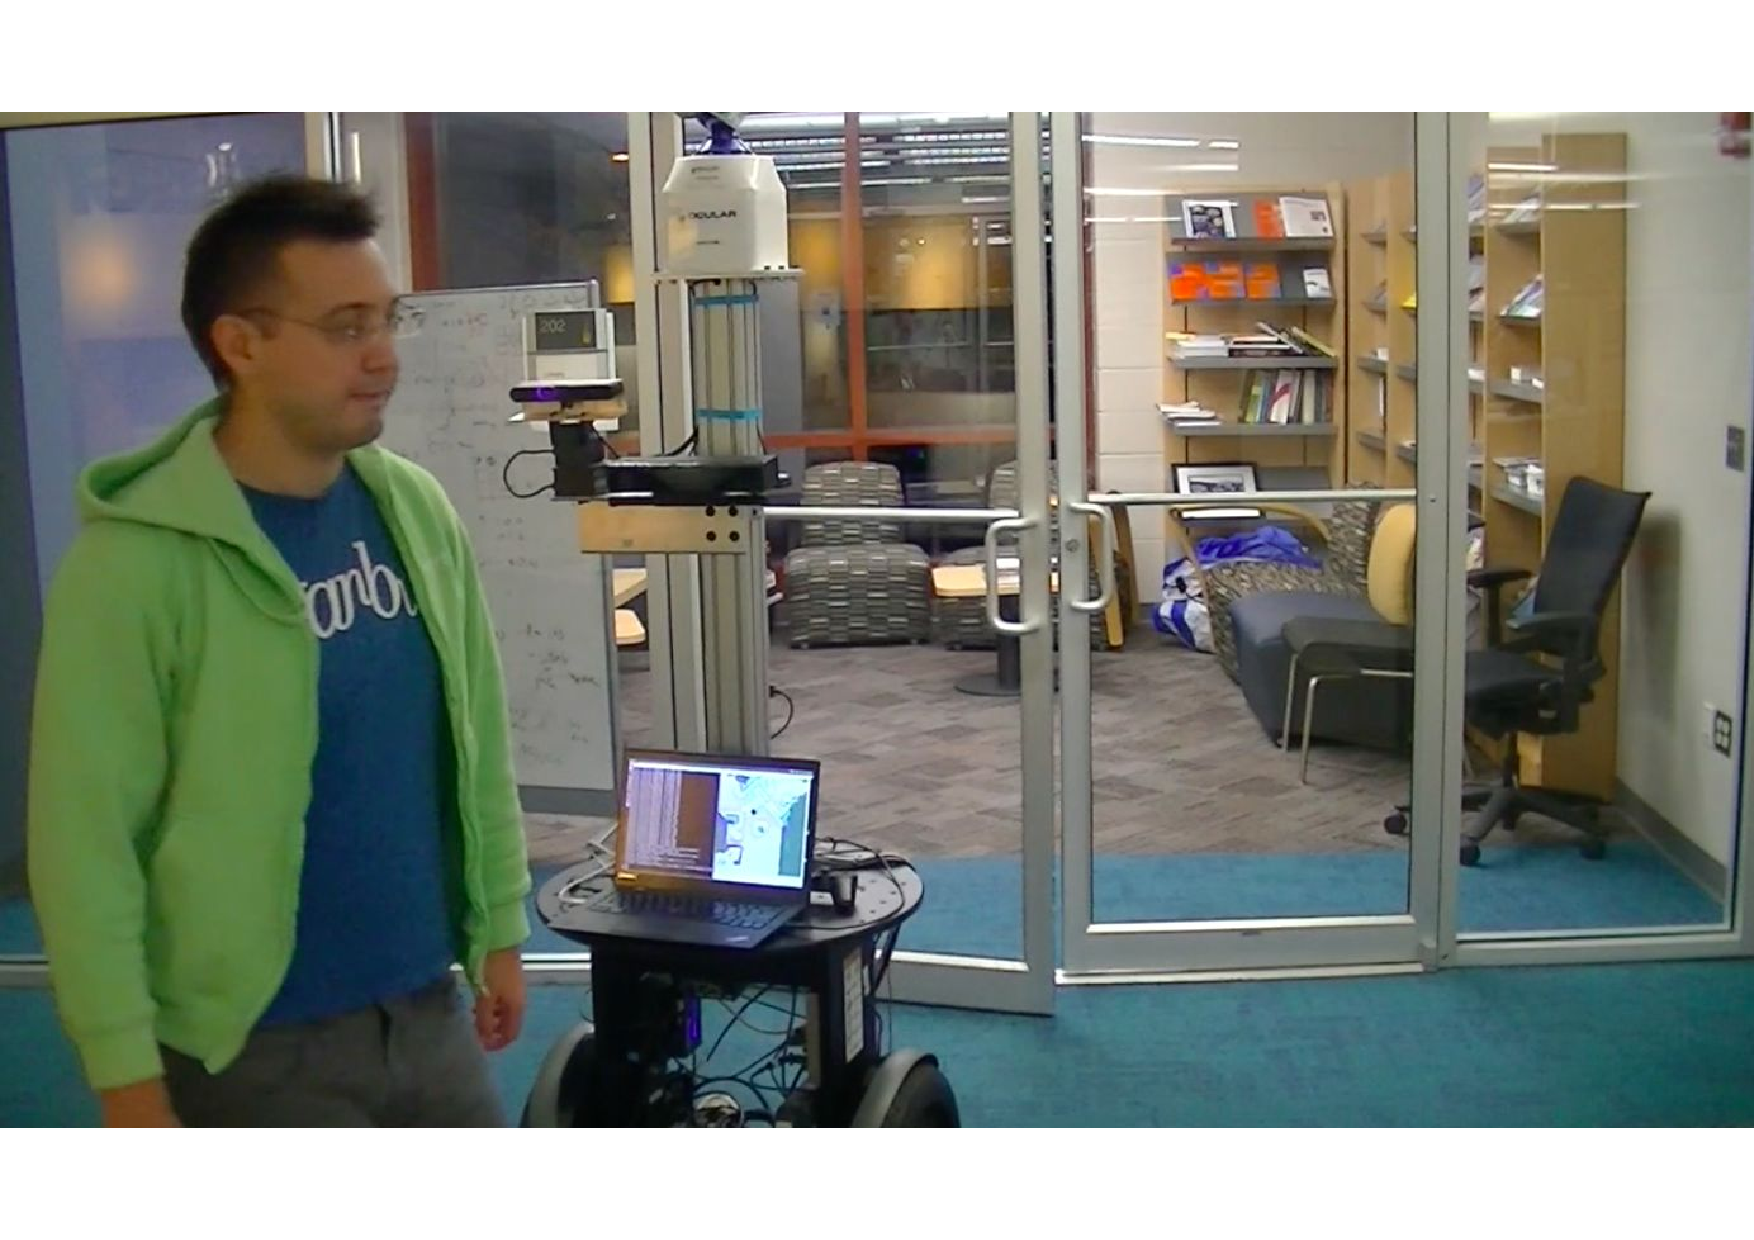
\includegraphics[width=0.49\textwidth]{pics/sit_door_04}
        }
    \caption{Demonstration of situation awareness for door passing during person following. It is assumed that the user previously added the door as a labeled landmark to the semantic map via the Tour Scenario. This is a swing door with spring loaded hinges, so it would close if not kept open actively. a) The robot is following the user by keeping a fixed distance in between. b) Signal phase: The user has stopped, is in close proximity to the door and performed a pointing gesture toward the other room. c) Approach Phase: The robot passes the door while the user is holding the door}
   \label{fig:situtation_aware_door_passing}
\end{figure}

A user may open, close or pass through a door, and detecting these actions beforehand requires a sophisticated recognition system. However the robot can assume that any of those actions are possible when the user is approacing the door. In our approach, the robot takes action when the user is nearby a door and performs a pointing gesture towards it, to signal that the robot should pass from the door (Signal Phase). If the action is not signaled, the robot continues with basic following during the door passage. The robot can continiously monitor the user's proximity to the doors using the semantic map, if the user labeled door landmarks beforehand. After the detection of a pointing gesture, a goal position is calculated (Approach Phase). The goal positions are sampled on the other side of the door, that is guaranteed not the block the opening/closing of the door. A collision-free position with the least obstacle cost sample is chosen as the goal point. Note that while the robot is moving, it does not necessarily keep a fixed distance to the user anymore. After the robot reaches the goal, it waits for the person to pass the door (Execution Phase). After the user moved away from the door, the basic following behavior takes over.  The phases and conditions for door passing situation are summarized in Table \ref{table:situation_aware_door_passing}. The situation awareness for this scenario is implemented on the Segway robot. The snapshots from the behavior can be seen in Figure \ref{fig:situtation_aware_door_passing}. Note that although our approach can handle doors with spring-loaded hinges, it does not have a model of the door except the convex hull of its plane.


\section{Application To Telepresence Robots}
\label{sec:following_application_to_telepresence}

A telepresence robot can be described as \textit{Skype on wheels}, where a remote user teleconferences while having the control of the movement of a robotic system in a physical environment. Telepresence robots constitute a promising area in the consumer robotics industry as evidenced by multiple start-up companies working on telepresence products. However, currently all the telepresence robots that are available in the market are controlled by manual driving - usually via the keyboard or a joystick. In this section, we present an implementation of person following on a telepresence robot and a user study that evaluates effect of having person following capability on a telepresence robot.

Telepresence robots are a level above video conferencing since the robot is used as the communication medium and the remote user can now control the movement. Therefore, the spatial interaction between people and a telepresence robot in social situations is worth investigating. One of those situations is moving with a group of people. In an effort to analyze the spatial and verbal interaction, we focus on engagement with one person where the remote user interacts with the person while following him/her in a corridor. This is situation is very likely to happen in office environments, for example when the remote user is having a discussion with a co-worker while walking to his office after a meeting. As telepresence robots become more common, there will be need to have the functionality of autonomous following of a person so that the remote user doesn't have to worry about controlling the robot.

We evaluate our system by conducting a user study, where there are two following conditions:

\begin{enumerate}
\item Manual Person Following: Robot is controlled with an Xbox controller
\item Autonomous Person Following: Initiated by clicking on a user in RGB-D image
\end{enumerate}

The aim of the user study is to measure how remote users like using the autonomous following feature compared to the manual. For the study, the remote user has a task that consists of listening to a passage the followed person reads and answering related questions after the interaction. We also observe subjects' experiences using the system, get useful feedback and pinpoint future challenges that can be helpful designing new applications for telepresence robots.

\subsection{Robot Platform}

\begin{figure}[h!]
\centering
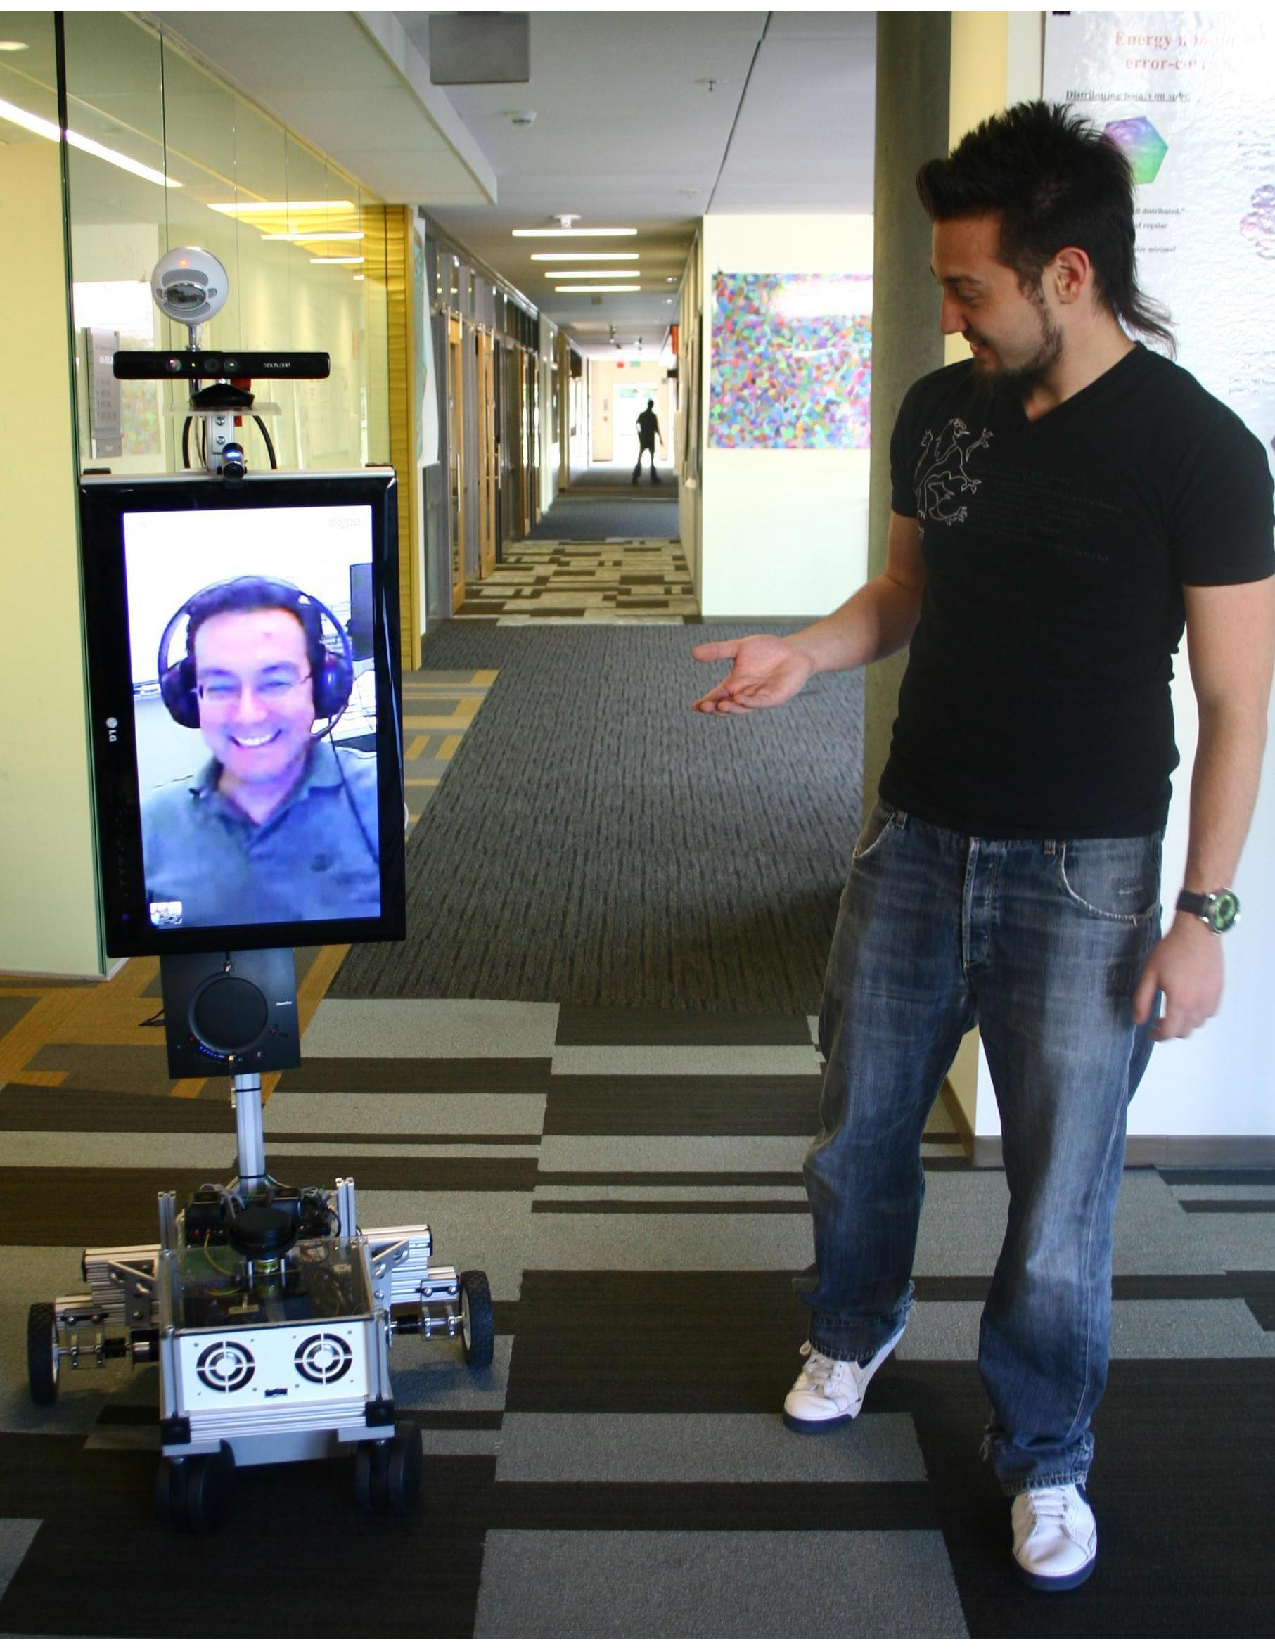
\includegraphics[width=0.4\textwidth]{pics/telepresence_robot}
\caption{The telepresence robot platform we used for our experiments.}
\label{fig:telepresence_robot}
\end{figure}

The system described in this paper is implemented on an experimental telepresence robot shown in Figure~\ref{fig:telepresence_robot}. The robot has a differential drive base and can be used for about 8 hours with full charge. For the experiments in this paper, the speed of the robot was limited to 0.55 m/s. A laser scanner with 360$^{\circ}$ field of view, which was taken from Neato XV-11 vacuum cleaning robot, was mounted horizontally at 0.3m height. The system runs on Windows 7 and Microsoft Robotics Developer Studio (MRDS) as its distributed computing environment. The remote user connects to the robot via wireless internet and communicates with others using Skype. On the remote end, . The robot is also equipped with an omni-directional microphone and a high-end speakerphone.

There are two operation modes for the robot: Teleoperation and Autonomous Person Following. A Xbox 360 Wireless Controller is used to remotely teleoperate the robot.  A wide-angle camera is placed on top of the monitor and tilted slightly downward to help the remote user to see the floor, robot base and people's faces at the same time. A Kinect Sensor is also placed above the monitor. Person following is initiated through the user interface shown in Figure \ref{fig:telepresence_ui}.

\begin{figure}[h!]
\centering
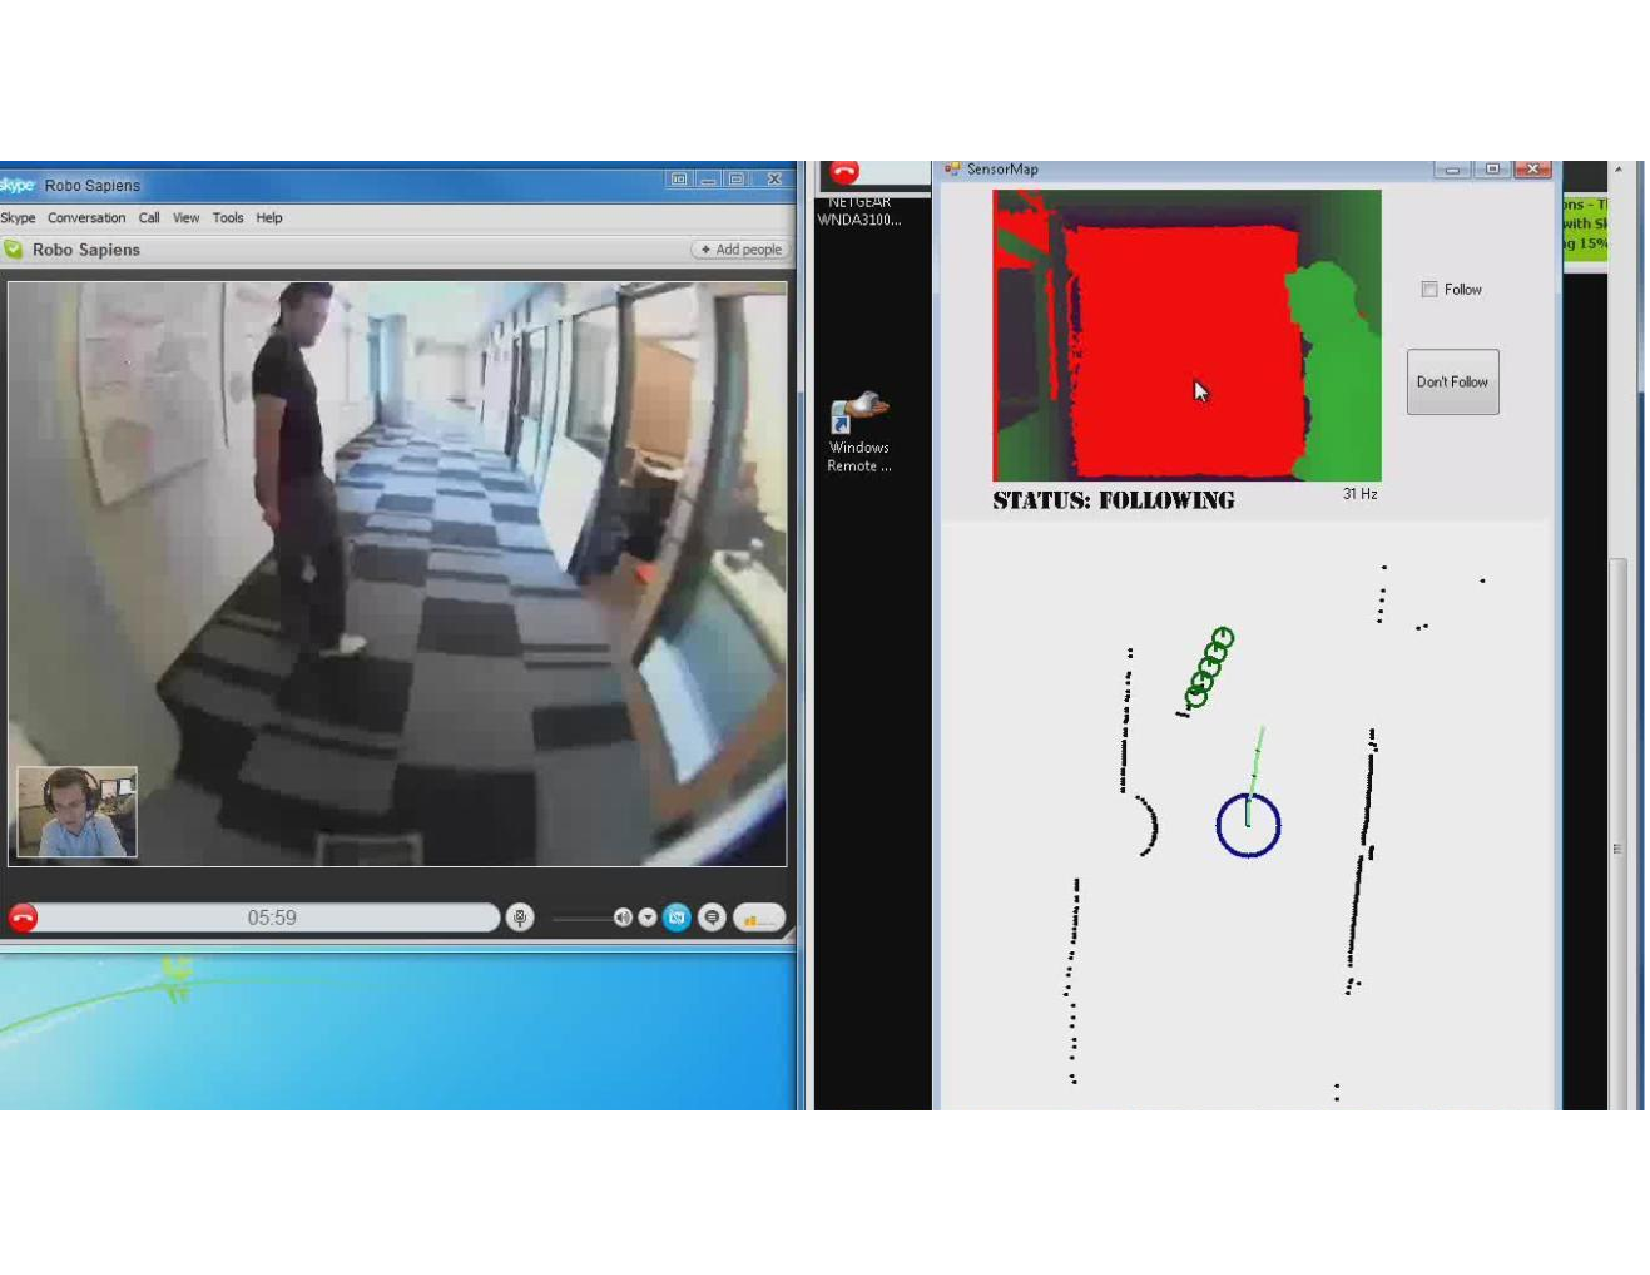
\includegraphics[width=1.0\textwidth]{pics/telepresence_ui_cropped}
\caption{User Interface of the robot for the remote user.}
\label{fig:telepresence_ui}
\end{figure}

A modified version of the local planner used in Section \ref{sec:navigation_local_planner} is used for person following. A utility function consisting multiple factors, including the respective position to the person, is optimized over multiple steps using Breadth-First Search. Details of the planning method can be found in \cite{cosgun2013autonomous}.

\subsection{User Study}

In this study, remote user is the subject and the followed person is the experimenter. To investigate the effectiveness of using autonomous person following for an interaction task, we ran a controlled experiment and varied manual vs. autonomous following within subjects.

\paragraph{Design:}
The experiments were conducted in working hours and bypassers were allowed to walk across the experiment area or talk. The subjects were given the task of following the experimenter through the course for a lap and listen to the passage he is reading. In the first run, the subject used the autonomous following or teleoperation method to follow a person and complete the lap. In the second run, the subject used the other method. At the end of each run, the subject was asked to complete a 4-question quiz about the passage. The passages and quiz questions were taken from Test of English as a Foreign Language (TOEFL) listening section examples. One passage was about ``behaviorism" and the other one was about ``manila hemps", and passages were chosen so that they are at a similar difficulty level. The time it takes to read a passage corresponded approximately to the same time a lap is completed. We also asked numbered 7 point Likert scale questions, administered after each run, about how \emph{Understandable} the experimenter was, \emph{Easiness of UI}, if the robot exhibited \emph {Natural Motions}, how \emph{Safe} the remote user felt, if the subject was able to \emph{Pay Attention} to the passage, how \emph{Fast} the robot was and how much \emph{Fun} the subject had. At the end of both runs, the user was asked which method he/she will prefer over the other for this type of a scenario. The exact questionnaire was show in Appendix \ref{chapter:telepresence_user_study_survey_questions}.

\paragraph{Participants:}

10 volunteers participated in the study (6 male and 4 female between the ages of 25-48). Participants consisted of 4 researchers and 6 interns at Microsoft Research. 5 of the participants had little knowledge, 4 had average knowledge and 1 had above average knowledge on robotics. The participants weren't gamers: 4 participants never played console games, 4 played rarely, 1 sometimes played and 1 often played. 6 of the participants often used video conferencing software, while 2 sometimes and 2 rarely used. 9 of the participants were not native English speakers and all of them had taken the TOEFL before. Participants were recruited through personal relations and were given a small gift (valued at approximately US$ \$ $10) for their help.

\paragraph{Procedure:}

The participants were first greeted by the experimenter and instructed to complete a pre-task questionnaire regarding their background. The robot was shown to the participant and basic information about its capabilities was told. The experimenter explained the task while walking with the participant in the corridor and showing the course to be followed. Participants were told that they should stay close to the experimenter while he is walking and there will be a quiz regarding the passage afterwards. The participant was informed that there are 2 operation modes: manual and autonomous person following.

Before the experiment started, the participant went through training for about 15 minutes. First, the participant learned the basic controls for the Xbox controller when he/she was nearby the robot. Then the participant was taken to the remote station, which was in a room about 20 meters away from the corridor area. The participant was informed about the UI and was shown how the autonomous following can be activated. Then a test run was executed, where the remote user followed the experimenter via teleoperation and had a conversation.

After the training, the actual run was executed using either the manual or autonomous method. When the lap was completed, first the passage quiz, then the survey questions were answered by the subject. Then the second experiment using the other method was executed, and the second passage quiz and survey questions were given to the subject. As the last question, the subject was asked to state his/her method of preference. Lastly, the participants were debriefed about the study and engaged in a discussion. We switched the starting method for every other experiment in order not to bias the subjects' opinions about one particular method.

\paragraph{Measures:}
We had three measurement criteria to compare manual vs autonomous following: 1) Number of correct answers to passage quizzes: Assuming the standardized TOEFL exercises were of same difficulty, we ran a paired $t-test$ on two groups of autonomous and manual. 2) Survey questions: We ran a paired $t-test$ using 7-point Likert Scale on each of the seven questions. 3) Preferred Method: We looked at which method subjects chose over the other one.

\paragraph{Results:}

Out of 4 quiz questions, the correct answers for autonomous group ($\mu=2.9$, $\sigma=0.9$) were more than the manual group ($\mu=2.2$, $\sigma=1.2$) but the statistical difference was not statistically significant ($t(9)=1.48$, $p=0.17$ on $t-test$).

\begin{table}
	\centering
  \begin{tabular}{lSSSSSS}    
    \toprule
    \multirow{2}{*}{Question} &
      \multicolumn{2}{c}{Autonomous} &
      \multicolumn{2}{c}{Manual Drive} &
      \multicolumn{2}{c}{$t-test$} \\
      & {$\mu$} & {$\sigma$} & {$\mu$} & {$\sigma$} & {$p$} & {$t$} \\
      \midrule
    1. Understandable & 4.0&	1.5&	3.6&	1.7&	0.47 & 0.73 \\
    2. Easy UI & 6.5&	0.9&	5.0&2.2&0.06& 2.13 \\
    3. Natural Motion &  5.4 & 1.0& 3.5 & 1.9 & 0.03 & 2.52 \\
    4. Safe & 5.1 & 1.7 & 2.3 & 1.4 & 0.01 & 3.09 \\
    5. Pay Attention & 5.3 & 1.8 & 3.4 & 1.5 & 0.02 & 2.63 \\
    6. Fast & 3.9 & 0.3 & 4.3 & 0.8 & 0.10 & -1.8 \\
    7. Fun & 5.3 & 1.5 & 5.1 & 1.7 & 0.66 & 0.45 \\
    \bottomrule
  \end{tabular}
      \caption{Survey results of the user study for person following for telepresence robots. Table displays survey question average and standard deviations for the two conditions: Autonomous Person Following and Manual Person Following.}
    \label{table:telepresence_table}
\end{table}


Table \ref{table:telepresence_table} summarizes the survey results. For \emph{Understandable} and \emph{Fun}, the scores slightly favored autonomous method but the difference wasn't statistically significant. Manual method User Interface (gaming controller) was found to be easy to use ($\mu=5.0$, $\sigma=2.2$), but the UI for autonomous method (clicking) was found to be marginally easier ($\mu=6.5$, $\sigma=0.9$), ($t(9)=2.13$, $p=0.06$). The motions of the robot was found to be significantly more \emph{Natural} to have a conversation for autonomous ($\mu=5.4$, $\sigma=1.0$) than manual ($\mu=3.5$, $\sigma=1.9$), ($t(9)=2.52$, $p=0.03$). Participants thought they were able to \emph{Pay more Attention} to the passage the experimenter is reading when the robot was following the him autonomously ($\mu=5.3$, $\sigma=1.8$) compared to manual control ($\mu=3.4$, $\sigma=1.5$) and the statistical difference was significant ($t(9)=2.63$, $p=0.02$). Participants have found the autonomous method ($\mu=5.1$, $\sigma=1.7$) much safer than manual method ($\mu=2.3$, $\sigma=1.4$) and there was a significant difference between two groups ($t(9)=3.09$, $p=0.01$). The speed of the robot was found to be neither fast nor slow for both methods ($\mu=3.9$, $\sigma=0.3$) and ($\mu=4.3$, $\sigma=0.8$).

All 10 subjects chose autonomous person following over teleoperation for this task.




\subsection{Design Implications}

Our user study showed that a person following behavior is desirable for telepresence robots when there is interaction. The follow-up discussions also agreed with the survey results, as one subject (R10) stated: \emph{``It just gives me more focus and concentration.''} Below, we list our observations and implications for future research and design for telepresence robots:

\textbf{Motor Noise:} Even though the motors on the robot were relatively quiet, 8 out of 10 participants expressed that the motor noise made communication harder. This justifies the close scores we collected in the survey question asking if the subject was able to understand what the experimenter was saying. (R8) was disturbed by the noise: \emph{``When I was driving, it was always this constant sound. It was worse for the autonomous one. It was constantly adjusting and compensating for the movement."} On the other hand, (R5) found the motor noise useful: \emph{``I actually like it because it gives me the feedback whether I'm driving faster or slower. It also gives me a little bit feeling of life."} Thus, although excessive motor noise should be avoided, some noise might be useful.

\textbf{Wireless Connection:} Second most cited problem for video conferencing was the video quality and time lags. (R8) clearly expressed why it was hard to walk with the experimenter using the manual method: \emph{``The frame rate drops all of a sudden and you have no choice but to stop."} Another subject (R9) made use of the displayed sensor data when the video conferencing quality went bad: \emph{``Because of the lag, I just switched to the Kinect (depth image) and the overhead view (laser)."} This was possible because the wide angle camera image was coming from Skype whereas sensor displays were received from the Windows Remote Assistance. Clearly, a big challenge for telepresence systems is to deal with wireless connection problems.

\textbf{Natural Interaction:} Even though the participants thought the motions of the robot were natural to have a conversation ($\mu=5.4$, $\sigma=1.0$), some didn't feel it was a natural way to communicate. As seen in Figure \ref{fig:telepresence_robot}, the screen displaying the remote user's face is flat and it introduced problems when the robot was traveling on the side of the person. (R5), when asked about walking side by side: \emph{``..we don't have face-to-face. It is not really a conversation."} This raises design considerations on how the remote user's face is brought out. One of the subjects (R5) discovered that the microphone characteristics are different than human hearing: \emph{``I don't have a distance sense if the experimenter is further away or close. If you have the fading audio, then I'll immediately notice."} Whether a telepresence robot should exhibit the same characteristics of human perception or not is an open question and needs further investigation.

\textbf{Assisted Teleoperation:} Telepresence robots should possess a layer to assists the remote user to avoid obstacles and collisions. \emph{Safety} ratings for the manual method were very low ($\mu=2.3$, $\sigma=1.4$) and (R8) expressed the concern: \emph{``I was especially worried about running into the experimenter."} This suggests that scenarios involving interaction would demand more attention of the remote users. The teleoperation should also be intuitive and be similar to driving modalities that people are already used to. (R4) stated: \emph{``I was thinking about Manual mode compared to driving a car."} before suggesting \emph{``.. maybe something like a cruise control might be good."}

\textbf{Gaming Experience:} Since the robot was controlled by a gaming console controller, some participants likened the manual mode to gaming. (R9) said: \emph{``Manual is like playing video games."} and (R5) said: \emph{``I don't play video games so controlling those consoles is not natural to me."} Thus, it is possible that gamers are less likely to have trouble driving the robot. This observation is also made by Takayama \cite{takayama2011assisted}.

\textbf{Long Term Interaction:} None of the subjects participated in our study had used a telepresence robot before. (R6) justified the inability to use the manual method: \emph{``Maybe if I have some more practice for about several hours of driving the robot, I can use manual as well as autonomous.''} (R8) on having fun using teleoperation: \emph{``It was fun because it was the first time I did it but I can imagine that over time, I'll get bored of it."} The \emph{Fun} question in the survey received similar scores for autonomous and manual, possibly because using a telepresence robot was a new experience for the subjects. Studies regarding long term interaction for telepresence robots can yield interesting results, as in \cite{lee2011now}.

\textbf{Error recovery:} When the person was lost during following, the UI displayed a text that the person was lost so that the remote user can re-initiate the following by clicking on the person. None of the subjects complained about the robot losing the person. When asked explicitly about the robot losing the experimenter, (R10) answered: \emph{``That's not a big deal in comparison to me driving the robot."} Therefore, applications developed for telepresence robots can take advantage of the human being in the loop and does not have to be error-free for deployment.

\subsection{Discussion}

User studies showed that autonomous person following
is a desired capability for a telepresence robot and it was
favored over direct teleoperation for an accompanying task.
Autonomous following was found to be safer, easier to use
and helped the remote users to pay more attention to the
conversation instead of the robot control. From the experience
earned from user studies, there are still interesting
challenges to explore in terms of human-robot interaction for
telepresence robots.

%%%%%%%%%%%%%%%%%%%%%%